% Options for packages loaded elsewhere
\PassOptionsToPackage{unicode}{hyperref}
\PassOptionsToPackage{hyphens}{url}
\PassOptionsToPackage{dvipsnames,svgnames,x11names}{xcolor}
%
\documentclass[
  12pt]{article}

\usepackage{amsmath,amssymb}
\usepackage{iftex}
\ifPDFTeX
  \usepackage[T1]{fontenc}
  \usepackage[utf8]{inputenc}
  \usepackage{textcomp} % provide euro and other symbols
\else % if luatex or xetex
  \usepackage{unicode-math}
  \defaultfontfeatures{Scale=MatchLowercase}
  \defaultfontfeatures[\rmfamily]{Ligatures=TeX,Scale=1}
\fi
\usepackage{lmodern}
\ifPDFTeX\else  
    % xetex/luatex font selection
\fi
% Use upquote if available, for straight quotes in verbatim environments
\IfFileExists{upquote.sty}{\usepackage{upquote}}{}
\IfFileExists{microtype.sty}{% use microtype if available
  \usepackage[]{microtype}
  \UseMicrotypeSet[protrusion]{basicmath} % disable protrusion for tt fonts
}{}
\makeatletter
\@ifundefined{KOMAClassName}{% if non-KOMA class
  \IfFileExists{parskip.sty}{%
    \usepackage{parskip}
  }{% else
    \setlength{\parindent}{0pt}
    \setlength{\parskip}{6pt plus 2pt minus 1pt}}
}{% if KOMA class
  \KOMAoptions{parskip=half}}
\makeatother
\usepackage{xcolor}
\setlength{\emergencystretch}{3em} % prevent overfull lines
\setcounter{secnumdepth}{5}
% Make \paragraph and \subparagraph free-standing
\ifx\paragraph\undefined\else
  \let\oldparagraph\paragraph
  \renewcommand{\paragraph}[1]{\oldparagraph{#1}\mbox{}}
\fi
\ifx\subparagraph\undefined\else
  \let\oldsubparagraph\subparagraph
  \renewcommand{\subparagraph}[1]{\oldsubparagraph{#1}\mbox{}}
\fi


\providecommand{\tightlist}{%
  \setlength{\itemsep}{0pt}\setlength{\parskip}{0pt}}\usepackage{longtable,booktabs,array}
\usepackage{calc} % for calculating minipage widths
% Correct order of tables after \paragraph or \subparagraph
\usepackage{etoolbox}
\makeatletter
\patchcmd\longtable{\par}{\if@noskipsec\mbox{}\fi\par}{}{}
\makeatother
% Allow footnotes in longtable head/foot
\IfFileExists{footnotehyper.sty}{\usepackage{footnotehyper}}{\usepackage{footnote}}
\makesavenoteenv{longtable}
\usepackage{graphicx}
\makeatletter
\def\maxwidth{\ifdim\Gin@nat@width>\linewidth\linewidth\else\Gin@nat@width\fi}
\def\maxheight{\ifdim\Gin@nat@height>\textheight\textheight\else\Gin@nat@height\fi}
\makeatother
% Scale images if necessary, so that they will not overflow the page
% margins by default, and it is still possible to overwrite the defaults
% using explicit options in \includegraphics[width, height, ...]{}
\setkeys{Gin}{width=\maxwidth,height=\maxheight,keepaspectratio}
% Set default figure placement to htbp
\makeatletter
\def\fps@figure{htbp}
\makeatother

\addtolength{\oddsidemargin}{-.5in}%
\addtolength{\evensidemargin}{-1in}%
\addtolength{\textwidth}{1in}%
\addtolength{\textheight}{1.7in}%
\addtolength{\topmargin}{-1in}%

\usepackage{booktabs}
\usepackage{longtable}
\usepackage{array}
\usepackage{multirow}
\usepackage{wrapfig}
\usepackage{float}
\usepackage{colortbl}
\usepackage{pdflscape}
\usepackage{tabu}
\usepackage{threeparttable}
\usepackage{threeparttablex}
\usepackage[normalem]{ulem}
\usepackage{makecell}
\usepackage{xcolor}
\makeatletter
\makeatother
\makeatletter
\makeatother
\makeatletter
\@ifpackageloaded{caption}{}{\usepackage{caption}}
\AtBeginDocument{%
\ifdefined\contentsname
  \renewcommand*\contentsname{Table of contents}
\else
  \newcommand\contentsname{Table of contents}
\fi
\ifdefined\listfigurename
  \renewcommand*\listfigurename{List of Figures}
\else
  \newcommand\listfigurename{List of Figures}
\fi
\ifdefined\listtablename
  \renewcommand*\listtablename{List of Tables}
\else
  \newcommand\listtablename{List of Tables}
\fi
\ifdefined\figurename
  \renewcommand*\figurename{Figure}
\else
  \newcommand\figurename{Figure}
\fi
\ifdefined\tablename
  \renewcommand*\tablename{Table}
\else
  \newcommand\tablename{Table}
\fi
}
\@ifpackageloaded{float}{}{\usepackage{float}}
\floatstyle{ruled}
\@ifundefined{c@chapter}{\newfloat{codelisting}{h}{lop}}{\newfloat{codelisting}{h}{lop}[chapter]}
\floatname{codelisting}{Listing}
\newcommand*\listoflistings{\listof{codelisting}{List of Listings}}
\makeatother
\makeatletter
\@ifpackageloaded{caption}{}{\usepackage{caption}}
\@ifpackageloaded{subcaption}{}{\usepackage{subcaption}}
\makeatother
\makeatletter
\@ifpackageloaded{tcolorbox}{}{\usepackage[skins,breakable]{tcolorbox}}
\makeatother
\makeatletter
\@ifundefined{shadecolor}{\definecolor{shadecolor}{rgb}{.97, .97, .97}}
\makeatother
\makeatletter
\makeatother
\makeatletter
\makeatother
\ifLuaTeX
  \usepackage{selnolig}  % disable illegal ligatures
\fi
\usepackage[]{natbib}
\bibliographystyle{agsm}
\IfFileExists{bookmark.sty}{\usepackage{bookmark}}{\usepackage{hyperref}}
\IfFileExists{xurl.sty}{\usepackage{xurl}}{} % add URL line breaks if available
\urlstyle{same} % disable monospaced font for URLs
\hypersetup{
  pdftitle={Visualising How Non-linear Dimension Reduction Warps Your Data},
  pdfauthor={Jayani P.G. Lakshika; Dianne Cook; Paul Harrison; Michael Lydeamore; Thiyanga S. Talagala},
  pdfkeywords={high-dimensional data, dimension
reduction, triangulation, hexagonal binning, low-dimensional
manifold, manifold learning, tour, data vizualization},
  colorlinks=true,
  linkcolor={blue},
  filecolor={Maroon},
  citecolor={Blue},
  urlcolor={Blue},
  pdfcreator={LaTeX via pandoc}}


\begin{document}


\def\spacingset#1{\renewcommand{\baselinestretch}%
{#1}\small\normalsize} \spacingset{1}

%%%%%%%%%%%%%%%%%%%%%%%%%%%%%%%%%%%%%%%%%%%%%%%%%%%%%%%%%%%%%%%%%%%%%%%%%%%%%%

\title{\bf Visualising How Non-linear Dimension Reduction Warps Your
Data}
\author{
Jayani P.G. Lakshika\\
Econometrics \& Business Statistics, Monash University\\
and\\Dianne Cook\\
Econometrics \& Business Statistics, Monash University\\
and\\Paul Harrison\\
MGBP, BDInstitute, Monash University\\
and\\Michael Lydeamore\\
Econometrics \& Business Statistics, Monash University\\
and\\Thiyanga S. Talagala\\
Statistics, University of Sri Jayewardenepura\\
}
\maketitle

\bigskip
\bigskip
\begin{abstract}
Non-Linear Dimension Reduction (NLDR) techniques have emerged as
powerful tools to visualize high-dimensional data. However, their
complexity and parameter choices may lead to distrustful or misleading
results. To address this challenge, we propose a novel approach that
combines the tour technique with a low-dimensional manifold generated
using NLDR techniques, hexagonal binning, and triangulation. This
integration enables a clear examination of the low-dimensional
representation in the original high-dimensional space. Our approach not
only preserves the advantages of both tours and NLDR but also offers a
more intuitive perception of complex data structures and facilitates
accurate data transformation assessments. The method and example data
sets are available in the \textbf{quollr} R package.
\end{abstract}

\noindent%
{\it Keywords:} high-dimensional data, dimension
reduction, triangulation, hexagonal binning, low-dimensional
manifold, manifold learning, tour, data vizualization
\vfill

\newpage
\spacingset{1} % DON'T change the spacing! (Default 1.9)

\ifdefined\Shaded\renewenvironment{Shaded}{\begin{tcolorbox}[sharp corners, interior hidden, enhanced, borderline west={3pt}{0pt}{shadecolor}, breakable, boxrule=0pt, frame hidden]}{\end{tcolorbox}}\fi

\hypertarget{sec-intro}{%
\section{Introduction}\label{sec-intro}}

High-dimensional (high-D) data is prevalent across various fields, such
as ecology and bioinformatics \citep{Guo2023}, due to advancements in
data collection technologies \citep{Johnstone2009, ayesha2020overview}.
However, visualization of high-D data introduces significant challenges,
because the complexity of visualizing data beyond two dimensions
\citep{Jia2022}. In recent years, interactive and dynamic graphics
systems like \textbf{liminal} \citep{article21} ---which employs
interactive tools like brushing and linking \citep{article58}---and
software tools such as \textbf{XGobi}, \textbf{GGobi} \citep{article60},
\textbf{tourr} \citep{article61}, \textbf{detourr} \citep{article22},
and \textbf{langevitour} \citep{article09}, involving dynamic methods
like tours \citep{Asimov1985}, have played a key role in visualizing
high-D data (data-vis).

To create low-dimensional representations (typically in 2D) (m-vis)
\citep{article59} of high-D data, it is common to apply dimension
reduction (DR) techniques. Approaches for DR involve linear methods such
as principal component analysis (PCA) \citep{Karl1901}, non-linear
methods such as multi-dimensional scaling (MDS) \citep{Torgerson1967}.
In the past decade, many new non-linear dimension reduction (NLDR)
techniques have emerged, such as t-distributed stochastic neighbor
embedding (tSNE) \citep{Laurens2008} and uniform manifold approximation
and projection (UMAP) \citep{Leland2018}. NLDR techniques are the 2D
models of high-D data in our context.

It is important to visualize various non-linear dimensionality reduction
(NLDR) techniques for the same high-D data in order to understand and
find the best representation. After doing so, the 2D models may differ
considerably from each other and may also deviate from the original data
structure in high-dimensional space. Therefore, visualizing the 2D model
in high-D space (m-in-ds) is more useful to answer different types of
questions:

\begin{itemize}
\item
  Is there a best 2D representation of high-D data or are they all
  providing equivalent information? Is there a best parameter choice to
  fit the 2D model? How does the model change when it's parameters
  change?
\item
  How well the does the 2D models capture the data structure? Is the
  model fitting able to capture different data structure like
  non-linear, clustering?
\end{itemize}

If we cannot easily ask and answer these questions, our ability to
understand the models is limited. To find the best 2D model and
parameter choices, a better understanding of the underlying science is
important.

Also, the importance of m-vis along with data-vis has been recognized
and incorporated into interactive software, \textbf{liminal}
\citep{article21}. But the 2D model and high-D visualize side by side
and interactive like brushing and linking connect the data in the two
panels. To address this challenge, we propose a novel approach by
combining the tour technique with a low-dimensional manifold. This
manifold is created through the synergistic use of NLDR techniques,
hexagonal binning, and triangulation. This integration facilitates a
more understanding of the data structure, how well (or how poorly) NLDR
techniques perform.

The outline of this paper is as follows. The
Section~\ref{sec-background} provides an detailed overview of dimension
reduction methods, and tours. Building upon this foundation, the
Section~\ref{sec-methods} delves into the proposed algorithm, its
implementation details, how to tune the model, model summaries, and a
synthetic example to illustrate the functionality of the algorithm.
Subsequently, Section~\ref{sec-applications} showcases applications of
the algorithm on different data sets, particularly in single-cell
RNA-seq data. These applications reveal insights into the performance
and trustworthiness of NLDR algorithms. We analyze the results to
identify situations where NLDR techniques may lead to misleading
interpretations. Finally, \textbf{?@sec-conclusions} concludes by
summarizing the findings and emphasizing the significance of the
proposed approach in tackling the challenges of high-dimensional data
visualization.

\begin{figure}

{\centering 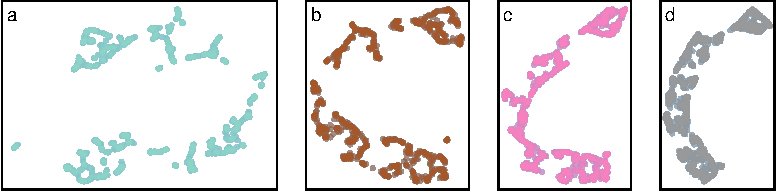
\includegraphics[width=1\textwidth,height=\textheight]{paper_files/figure-pdf/fig-nldervisUMAP-1.pdf}

}

\caption{\label{fig-nldervisUMAP}2D layouts from UMAP applied for the
S-curve data: (a) UMAP (n\_neighbors = 7), (b) UMAP (n\_neighbors = 15),
(c) UMAP (n\_neighbors = 32), (d) UMAP (n\_neighbors = 50). Is there a
best hyperparameter choice in representing UMAP or are they all
providing equivalent information?}

\end{figure}

\hypertarget{sec-background}{%
\section{Background}\label{sec-background}}

\hypertarget{dimension-reduction}{%
\subsection{Dimension Reduction}\label{dimension-reduction}}

Consider the high-D data a rectangular matrix \(X_{n \times p}\), where
\(X_{n \times p} = \begin{bmatrix} \textbf{x}_{1} & \textbf{x}_{2} & \cdots & \textbf{x}_{n}\\ \end{bmatrix}^\top\),
with \(n\) observations in \(p\) dimensions. The objective is to
discover a low-dimensional projection
\(Y_{n \times d} = \begin{bmatrix} \textbf{y}_{1} & \textbf{y}_{2} & \cdots & \textbf{y}_{n}\\ \end{bmatrix}^\top\),
represented as an \(n\) × \(d\) matrix, where \(d \ll p\). The reduction
process seeks to remove noise from the original data set while retaining
essential information.

There are two main categories of dimension reduction techniques: linear
and non-linear methods. Linear techniques involve a linear
transformation of the data, with one popular example being PCA. PCA
performs an eigen-decomposition of the sample covariance matrix to
obtain orthogonal principal components that capture the variance of the
data \citep{Karl1901}.

In contrast, NLDR techniques generate the low-dimensional representation
\(Y\) from the high-dimensional data \(X\), often using pre-processing
techniques like \(k\)-nearest neighbors graph or kernel transformations.
Multidimensional Scaling (MDS) is a class of NLDR methods that aims to
construct an embedding \(Y\) in a low-dimensional space, approximating
the pair-wise distances in \(X\) \citep{Torgerson1967}. Variants of MDS
include non-metric scaling \citep{article62} and Isomap, which estimate
geodesic distances to create the low-dimensional representation
\citep{article63}. Other approaches based on diffusion processes, like
diffusion maps \citep{article64} and the PHATE (Potential of
Heat-diffusion for Affinity-based Trajectory Embedding) algorithm
\citep{article03}, also fall under NLDR methods.

\hypertarget{non-linear-dimension-reduction-techniques}{%
\subsubsection{Non-linear dimension reduction
techniques}\label{non-linear-dimension-reduction-techniques}}

NLDR techniques are crucial for analyzing and displaying
high-dimensional data, where linear approaches may not adequately
capture complexities in relationships between variables
\citep{Johnstone2009}. One of the challenges with NLDR techniques is the
selection and tuning of appropriate hyperparameters \citep{liao2023}.
This process involves finding the suitable combination of
hyperparameters that enhances the performance of the NLDR technique,
considering the characteristics of the dataset and the specific goals of
the analysis.

Additionally, another challenge is lack of reverse mapping. Techniques
like PCA and auto-encoders \citep{article65} provide a way to map back
from the low-dimensional space to the high-D space, facilitating data
reconstruction. However, some NLDR methods, such as tSNE, don't have a
specific way to reconstruct the original data from the low-dimensional
space.

In this article, mainly focus on five NLDR techniques. They are tSNE,
UMAP, PHATE, TriMAP \citep{article02}, and Pairwise Controlled Manifold
Approximation (PaCMAP) \citep{Yingfan2021}.

Among these, tSNE \citep{Laurens2008} stands out for its ability to
preserve pairwise distances. By minimizing the divergence between
probability distributions in both high and low-dimensional spaces, tSNE
effectively uncovers intricate structures and patterns within the data.
Its application is widespread, particularly in tasks requiring the
visualization of clusters and local relationships. However, achieving
effective results requires careful consideration of hyperparameters,
such as perplexity.

UMAP \citep{Leland2018} is a useful technique for simplifying data while
maintaining both local and overall structures. It builds a fuzzy
topological view by considering nearby data points and then optimizes a
simplified version to match that view. UMAP is known for working well
with different scales of relationships in data and is efficient in
handling large datasets. However, it's important to choose parameters
like neighbors and minimum distance carefully, as they can affect the
results.

Furthermore, PHATE \citep{article03} is great for understanding how
things develop, especially in single-cell genomics. It uses a heat
diffusion process to capture relationships between data points, like
points along a trajectory. While PHATE is excellent for revealing these
developmental structures, it requires careful tuning of its parameters
because of its specialized focus.

Additionally, TriMAP \citep{article02} takes a special approach by
creating a triangulated graph representation of the data. This method is
good at understanding both local and global structures by treating the
data as a network of triangles. TriMAP is powerful in capturing
complicated structures, but it's important to choose parameters
carefully, like deciding how many neighbors to consider.

PaCMAP \citep{Yingfan2021} is different because it adds supervised
learning to make a 2D representation while keeping the relationships
between pairs of points. It builds a graph using distances between pairs
and then makes the 2D representation better using a customizable loss
function. What's special about PaCMAP is that it can use class labels or
extra information to guide how it makes the 2D representation. This
gives users a way to change how PaCMAP works to fit their needs better.

\begin{figure}

{\centering 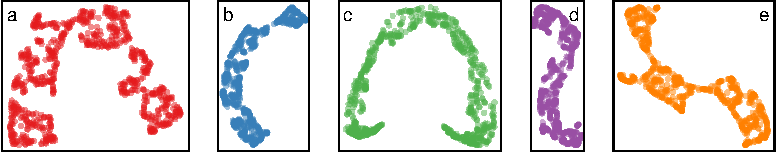
\includegraphics[width=1\textwidth,height=\textheight]{paper_files/figure-pdf/fig-nldervis-1.pdf}

}

\caption{\label{fig-nldervis}2D layouts from different NLDR techniques
applied the same data: (a) tSNE (perplexity = 27), (b) UMAP
(n\_neighbors = 50), (c) PHATE (knn = 5), (d) TriMAP (n\_inliers = 5,
n\_outliers = 4, n\_random = 3), and (e) PaCMAP (n\_neighbors = 10, init
= random, MN\_ratio = 0.9, FP\_ratio = 2). Is there a best
representation of the original data or are they all providing equivalent
information?}

\end{figure}

\hypertarget{linear-overviews-using-tours}{%
\subsection{Linear overviews using
tours}\label{linear-overviews-using-tours}}

A tour is a powerful visualization technique used to explore the shape
and global structure of high-dimensional data by generating a sequence
of projections, typically into two dimensions. There are two main types
of tours: the grand tour \citep{Asimov1985} and the guided tour
\citep{article29}. A grand tour involves randomly selecting new
orthonormal bases, enabling users to understand the structure by
exploring the subspace of d-dimensional projections \citep{Asimov1985}.
In contrast, a guided tour can be employed to generate a sequence of
`interesting' projections based on an index function \citep{article29}.

The process begins with the data matrix \(X\). It generates a sequence
of \(p\) × \(d\) orthonormal projection matrices (bases) \(P_t\),
usually \(d\) is one or two dimensions. For each pair of orthonormal
bases \(P_t\) and \(P_{t+1}\), a geodesic path is interpolated to create
smooth animation between projections. The resulting tour continuously
visualizes the projected data \(Y_t\) = \(XP_t\) as it interpolates
between successive bases.

Furthermore, software like \textbf{langevitour} can visualize both types
of tours, providing flexibility for exploring high-dimensional data with
various objectives. In our context, use grand tour along with the model
to observe how effectively the model captures the underlying structure
of the data.

\hypertarget{sec-methods}{%
\section{Methodology}\label{sec-methods}}

In this paper, we introduce a novel method to determine the most
effective NLDR technique and the best hyperparameter choice that
provides the most useful representation of high-D data. Our approach
involves dividing the high-D dataset into two parts: a training set for
constructing the model and a test set for generating predictive values
and residuals. Our algorithm takes a 2D embedding data as the input and
generate a tour that displays the high-D wireframe to overlay the data.
The flow chart of the proposed algorithm is shown in
Figure~\ref{fig-meth}. The algorithm consists of two main phases: (1)
generating the model in the 2D space and (2) lifting the model into
high-D space. The main steps of the algorithm are described in detail in
this section using UMAP 2D embedding of the S-curve dataset. This
dataset has seven dimensions, including four noise dimensions that were
added to the original 3D data.

\begin{figure}

{\centering 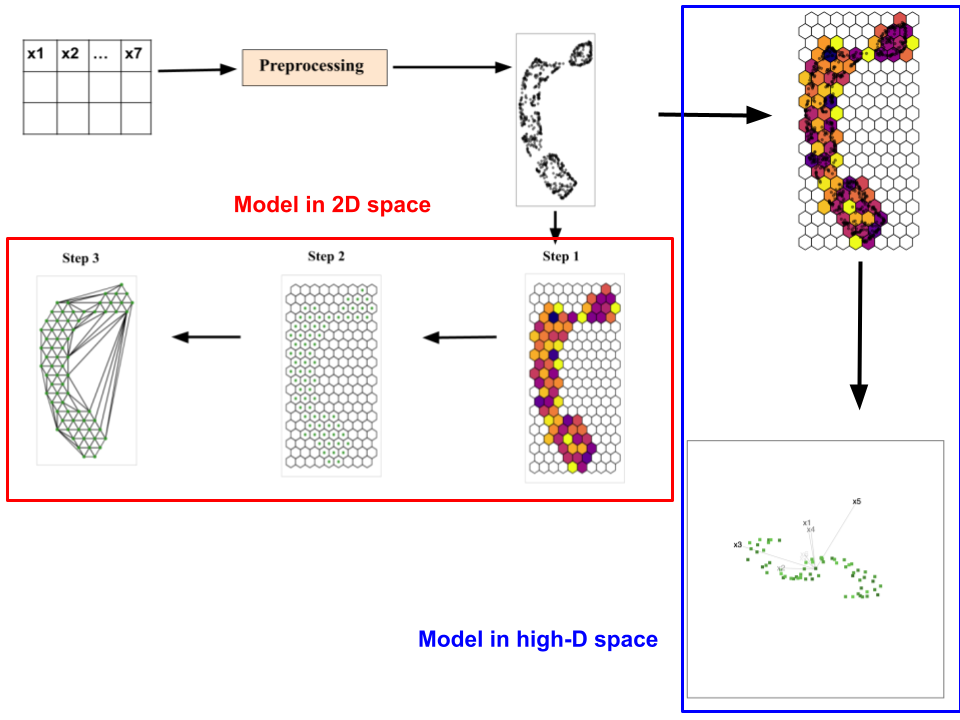
\includegraphics[width=1\textwidth,height=1\textheight]{figures/workflow.png}

}

\caption{\label{fig-meth}The flow diagram shows the main steps of our
algorithm. There are two basic phases, one to generate the model in the
2D space, and other to map the model into the high-D space.}

\end{figure}

\hypertarget{preprocessing-steps}{%
\subsection{Preprocessing steps}\label{preprocessing-steps}}

To reduce computational complexity when applying NLDR techniques to
high-D data and to reduce noise presence, PCA \citep[\citet{article68},
\citet{article69}]{article67} is used as a preprocessing step. PCA
involves identifying principal components that maximize variance. These
components are then used as the high-D data for the algorithm.

\hypertarget{sec-construct2d}{%
\subsection{Constructing the 2D model}\label{sec-construct2d}}

\textbf{Step 1: Scaling NLDR data}

First, we prepare the 2D embedding data to fit within the bounds
required for regular hexagonal binning. To achieve this, we implement
two key scaling steps. Scale the first 2D embedding component to range
between \(0\) and \(1\), ensuring that all data points fall within this
normalized interval. Secondly, we scale the second 2D embedding
component to range between \(0\) and \(y_{max}\) (see
Equation~\ref{eq-equation3}).

The calculation of \(y_{max}\) involves several steps. First, the aspect
ratio (\(ar\)) is computed by dividing the range of the second 2D
embedding component (\(r_2\)) by the range of the first 2D embedding
component (\(r_1\)) (see Equation~\ref{eq-equation1}). Then, the hexagon
ratio (\(hr\)) is determined by dividing the height of the hexagon
(\(hb\)) by its width (\(wb\)) (see Equation~\ref{eq-equation2}).
Finally, \(y_{max}\) is derived by taking the ceiling of
\(\frac{ar}{hr}\) and multiplying it by \(hr\). This process ensures
that \(y_{max}\) is an integer multiple of \(hr\), accommodating the
grid layout of the hexagonal bins.

\begin{equation}\protect\hypertarget{eq-equation1}{}{
 ar = \frac{r_2}{r_1}
}\label{eq-equation1}\end{equation}

\begin{equation}\protect\hypertarget{eq-equation2}{}{
 hr = \frac{hb}{wb}
}\label{eq-equation2}\end{equation}

\begin{equation}\protect\hypertarget{eq-equation3}{}{
 y_{max} = \left\lceil\frac{ar}{hr}\right\rceil * hr
}\label{eq-equation3}\end{equation}

\textbf{Step 2: Hexagonating NLDR data}

Hexagonating NLDR data (see Figure~\ref{fig-meth} Step 2) involves
partitioning the NLDR data into hexagonal bins, a technique commonly
referred to as hexagonal binning \citep[\citet{article66}]{Carr1987}.
This method use a hexagonal grid to create a bivariate histogram that
effectively visualizes the structure of high-D data. Hexagons, one of
only three regular polygons capable of tessellating a plane
\citep{Carr2013}, offer unique advantages due to their symmetry of
nearest neighbors and maximal number of sides for such tessellations
\citep{Dan2023}. This geometric property makes hexagons more efficient
in covering the plane compared to other regular tessellations and
reduces visual bias when displaying data densities \citep{Dan2023}.

In our algorithm, we aim to conduct regular hexagonal binning, involving
the computation of hexagonal grid configurations, the generation of the
grid, and the assignment of the NLDR data points to hexagons.

\textbf{(a) Computation of hexagonal grid configurations}

In the computation of hexagonal bin configurations, there are mainly two
configurations to consider: the number of bins along the x and y axes.
The first step involves in determining the hexagonal size (\(s\)) and
the buffer along the x and y axes (\(buffer_{x}\) and \(buffer_{y}\)).
Here, the hexagonal size (\(s\)) represents the radius of the outer
circle surrounding the hexagon. The buffer is important in expanding the
boundary to accommodate potential outliers or edge cases.

When computing the number of bins along the x and y axes (\(b_1\) and
\(b_2\)), the process begins by calculating the range of the respective
2D embedding component. After that, the range is adjusted to accommodate
the buffer amount. Then, the spacing between hexagons is determined
based on \(s\). Finally, the number of bins along the axis is computed
by dividing the adjusted range by the spacing.

For the computation of the number of bins along the x-axis (\(b_1\))
(see Equation~\ref{eq-equation12}), the range of the first embedding
component is defined as \(r_1\), while the buffer amount along the
x-axis is denoted as \(buffer_{x}\), and the horizontal spacing is
represented by \(h\) (see Equation~\ref{eq-equation11}). On the other
hand, the number of bins along the y-axis (\(b_2\)) (see
Equation~\ref{eq-equation14}) is computed based on the range of the
second embedding component (\(r_2\)), the buffer amount along the y-axis
(\(buffer_{y}\)), and the vertical spacing (\(v\)) (see
Equation~\ref{eq-equation13}).

\begin{equation}\protect\hypertarget{eq-equation11}{}{
 h = \sqrt{3} * s
}\label{eq-equation11}\end{equation}

\begin{equation}\protect\hypertarget{eq-equation12}{}{
 b_1 = \frac{r_1 + buffer_{x}}{h}
}\label{eq-equation12}\end{equation}

\begin{equation}\protect\hypertarget{eq-equation13}{}{
  v = 1.5 * s
}\label{eq-equation13}\end{equation}

\begin{equation}\protect\hypertarget{eq-equation14}{}{
 b_2 = \frac{r_2 + buffer_{y}}{v}
}\label{eq-equation14}\end{equation}

\textbf{(b) Generation of the hexagonal grid}

In this process, the first step involves generating centroids within the
hexagonal grid. This begins by defining the starting coordinates for the
hexagons. With the number of bins computed along the x and y axes, along
with the horizontal and vertical spacing, the centroids are iteratively
computed starting from the hexagonal starting coordinates.

Once the centroids for the hexagonal grid are obtained, the next step is
to compute the hexagonal coordinates. For example, if the centroid of a
hexagonal bin is defined as \((C_x, C_y)\), the hexagonal coordinates
can be computed using \(d_x\) (see Equation~\ref{eq-equation15}) and
\(d_y\) (see Equation~\ref{eq-equation16}) (see
Figure~\ref{fig-hexcoord}).

\begin{equation}\protect\hypertarget{eq-equation15}{}{
d_x = \frac{h}{2}
}\label{eq-equation15}\end{equation}

\begin{equation}\protect\hypertarget{eq-equation16}{}{
d_y = \frac{2* v * 1.15}{\sqrt{3}} 
}\label{eq-equation16}\end{equation}

\begin{figure}[H]

{\centering 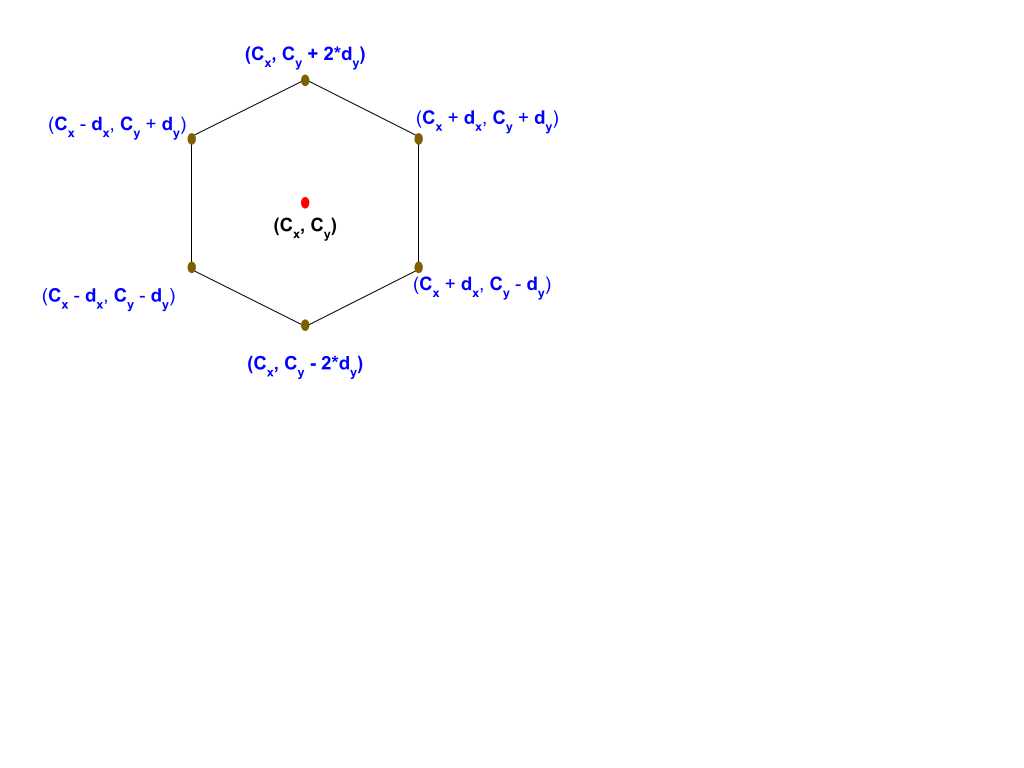
\includegraphics[width=1\textwidth,height=1\textheight]{figures/hex_coord.png}

}

\caption{\label{fig-hexcoord}The hexagonal coordinates computed for the
centroid \((C_x, C_y)\).}

\end{figure}

\textbf{(c) Assignment of the NLDR data points to hexagons}

After obtaining the centroids of the hexagonal bins for the entire grid,
the process of assigning NLDR points to hexagons involves determining
the nearest hexagonal bin for each NLDR point using the 2D Euclidean
distance. Then, the hexagonal ID of the nearest hexagon is assigned to
the corresponding NLDR points.

\textbf{Step 3: Obtaining bin centroids or bin means}

In the previous step, the algorithm clusters the 2D embedding data into
hexagons. Following this, in this step, the bin centroids or bin means
(see Figure~\ref{fig-meth} Step 3) are obtained \citep{Carr2013}.

The bin centroid (\(C_k^{(2)}\)) for a \(k^{th}\) hexagon with hexagonal
grid coordinates \((h^{k}x_{i}, h^{k}y_{i})\), where \(i = 1 \dots 6\)
can be defined as:

\begin{equation}\protect\hypertarget{eq-equation4}{}{
C_k^{(2)} = (C_{ky_1}, C_{ky_2}) = \left(\frac{\sum_{i=1}^{6} h^{k}x_{i}}{6}, \frac{\sum_{i=1}^{6} h^{k}y_{i}}{6}\right).
}\label{eq-equation4}\end{equation}

Also, the bin mean (\(C_k^{(2)}\)) is defined as the mean of the data
points within the \(k^{th}\) hexagon (see Equation~\ref{eq-equation5}).

\begin{equation}\protect\hypertarget{eq-equation5}{}{
C_k^{(2)} = (C_{ky_1}, C_{ky_2}) = \left(\frac{1}{n_k} \sum_{i=1}^{n_k} y_{1i}, \frac{1}{n_k} \sum_{i=1}^{n_k} y_{2i}\right),
}\label{eq-equation5}\end{equation}

where \(n_k\) is the number of data points within the hexagon,
\(y_{1i}\) and \(y_{2i}\) are the \(x\) and \(y\) coordinates of the
\(i^{th}\) data point within the hexagon.

\textbf{Step 4: Triangulating bin centroids or bin means}

In this step, the algorithm proceeds to triangulate the hexagonal bin
centroids or bin means (see Figure~\ref{fig-meth} Step 4). Triangulation
is a fundamental process in computational geometry and computer graphics
that involves dividing a set of points in a given space into
interconnected triangles \citep{article30}. One common algorithm used
for triangulation is Delaunay triangulation
\citep[\citet{article54}]{article26}, where points are connected in a
way that maximizes the minimum angles of the resulting triangles,
leading to a more regular and well-conditioned triangulation.

Delaunay triangulation can be defined as follows:

Let \(C^{(2)} = \{C_1^{(2)}, C_2^{(2)}, ..., C_m^{(2)}\}\) be a set of
\(m\) bin centroids or bin means in the plane. Delaunay triangulation of
\(C^{(2)}\), denoted as \(DT(C^{(2)})\), is a triangulation of the
convex hull of \(C^{(2)}\) such that the circumcircle of every triangle
in the triangulation contains no other points from \(C^{(2)}\).

Given that the hexagons are regular, the resulting triangles will mostly
be equilateral.

\hypertarget{lifting-the-model-into-high-dimensions}{%
\subsection{Lifting the model into high
dimensions}\label{lifting-the-model-into-high-dimensions}}

\hypertarget{lifting-the-triangular-mesh-points-into-high-dimensions}{%
\subsubsection{Lifting the triangular mesh points into high
dimensions}\label{lifting-the-triangular-mesh-points-into-high-dimensions}}

Consider \(f: \mathbb{R}^p \rightarrow \mathbb{R}^2\) be a function that
maps the high-D data (\(X_{n \times p}\)) to its NLDR equivalent
(\(Y_{n \times d}\)). Then, let
\(g: \mathbb{R}^2 \rightarrow \mathbb{R}^2\) be a function that maps
each 2D embedding point to its closest centroid (\(C^{(2)}\)). It
follows that \(f(g(x))\) maps the high-D points \(x\) to the centroid in
2D (\(C_k^{(2)}\)). Also, define a function
\(v: \mathbb{R}^2 \rightarrow \mathbb{R}^p\) maps the 2D centroid
(\(C^{(2)}\)) to the high-D mean of the points (\(C^{(p)}\)) in the
hexagon.

The high-D mean of all the points in \(k^{th}\) hexagon by

\begin{equation}\protect\hypertarget{eq-equation6}{}{
C_k^{(p)} = (C_{kx_1}, ..., C_{kx_p}) = \left(\frac{1}{n_k} \sum_{i=1}^{n_k} x_{1i}, \frac{1}{n_k} \sum_{i=1}^{n_k} x_{2i}, \dots ,\frac{1}{n_k} \sum_{i=1}^{n_k} x_{pi}\right).
}\label{eq-equation6}\end{equation}

Therefore,

\begin{equation}\protect\hypertarget{eq-equation7}{}{
v(C_k^{(2)}) = C_k^{(p)}.
}\label{eq-equation7}\end{equation}

Therefore, \(f(g(x))\) gives the 2D centroid associated with high-D
points \(x\), and \(v(C_k^{(2)})\) gives the high-D centroid associated
with 2D point \(C_k^{(2)}\). Thus, \(v(f(g(x)))\) gives the high-D
centroid (\(C_k^{(p)}\)) associated with the 2D embedding of the points
\(x\).

\hypertarget{lifting-the-2d-triangular-mesh-into-high-dimensions}{%
\subsubsection{Lifting the 2D triangular mesh into high
dimensions}\label{lifting-the-2d-triangular-mesh-into-high-dimensions}}

As described in Step 4 of Section~\ref{sec-construct2d}, during the
triangulation process in 2D space, vertices are identified to form
edges. With the knowledge of the high-D mappings for the 2D hexagonal
bins, the vertices connected in 2D are also connected in high-D (see
video linked in Figure~\ref{fig-wkhighD}).

\begin{figure}

{\centering 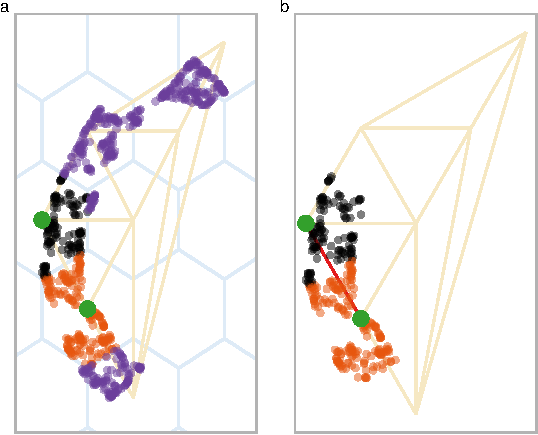
\includegraphics{paper_files/figure-pdf/fig-wkhighD-1.pdf}

}

\caption{\label{fig-wkhighD}How the 2D model lift into high dimensions?
(a) visualize the points and the hexagonal bin centroids related
\(7^{th}\) and \(12^{th}\) hexagons, (b) visualization of the edge
connected the \(7^{th}\) and \(12^{th}\) hexagons (colored in red) in
the triangular mesh. A video of tour animation is available at
\url{https://youtu.be/hxU91xNTJL0}.}

\end{figure}

\hypertarget{tuning-the-model}{%
\subsection{Tuning the model}\label{tuning-the-model}}

The performance and robustness of our model depend on four key
parameters: (i) the total number of bins (\(b\)), (ii) a benchmark value
used to remove low-density hexagons, (iii) a benchmark value used to
remove long edges, and (iv) starting point of the hexagonal grid.
However, there is no analytical formula to calculate an appropriate
value for these parameters (the computation of default values can be
find in \emph{quollr} paper). The selection of these parameter values
depends on the model performance computed by Mean Squared Error (MSE)
(see Section~\ref{sec-goodfit}).

\hypertarget{total-number-of-bins}{%
\subsubsection{Total number of bins}\label{total-number-of-bins}}

The number of hexagonal bins in the hexagonal grid has a considerable
impact on the construction of the 2D model. This is because it is the
initial step in building the 2D model. The hexagonal grid with the
chosen total number of bins must be able to capture the structure of the
NLDR data. If the number of bins is too low, the model may not be able
to capture the structure of the NLDR data effectively (see
Figure~\ref{fig-binsize} (a)), while if there are too many bins, it may
result in over-fitting the individual points of the NLDR data (see
Figure~\ref{fig-binsize} (c)). Therefore, it is important to determine
an appropriate number of bins to build an effective model.

\begin{figure}[H]

{\centering 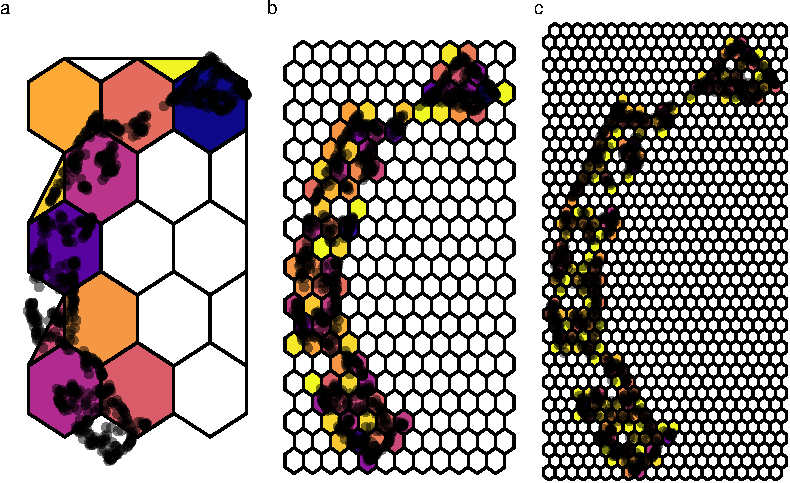
\includegraphics{paper_files/figure-pdf/fig-binsize-1.pdf}

}

\caption{\label{fig-binsize}Hexbin plots from different number of bins
for the \textbf{UMAP} embeddings of \textbf{S-curve} training data: (a)
b = 12 (3, 4), s = 0.62, (b) b = 84 (6, 14), s = 0.13, and (c) b = 336
(12, 28), s = 0.06. The hexbins are colored based on the density of
points, with darker colors indicating higher point density and yellow
color representing lower point density within each bin. What is the
number of bins that would be effective in representing low-dimensional
data?}

\end{figure}

\begin{equation}\protect\hypertarget{eq-equation8}{}{
b = b_1 \times b_2
}\label{eq-equation8}\end{equation}

Furthermore, the total number of bins is determined by the number of
bins along the x-axis and y-axis (see Equation~\ref{eq-equation8}). To
calculate the effective total number of bins, candidate values are
selected based on the range between the minimum and approximate maximum
number of bins along the x and y axes. The minimum number of bins along
each axis is set to \(1\), while the maximum number is estimated by
taking the square root of the NLDR data point count. The analysis
evaluates the MSE across varying total bin counts within this range,
covering the minimum to maximum values along both axes.

The analysis focuses on exploring the effect of total number of bins on
MSE. It considers MSE across different total number of bins, covering
the range calculated from the minimum to maximum values along both x and
y axes.

Typically, the MSE plot tends to have a steep slope at the beginning,
indicating that a smaller number of bins causes a larger amount of
error. Then, the slope gradually declines or levesl off, indicating that
a higher number of bins generates a smaller error. This MSE plot is
useful in determining the effective number of bins required to construct
the 2D model. Figure~\ref{fig-diagnosticpltScurve} has created a graph
that shows how the Mean Squared Error (MSE) changes depending on the
number of bins assigned in the hexagonal grid for UMAP applied to the
S-curve dataset. As per the rule of thumb mentioned earlier, the
effective number of bins is determined to be \(84\), with \(6\) bins
along the x-axis and \(14\) bins along the y-axis. Furthermore,
Figure~\ref{fig-modelScurve} shows the 2D model constructed using UMAP
with the selected total number of bins and how the model overlay on
high-D data.

\begin{figure}

{\centering 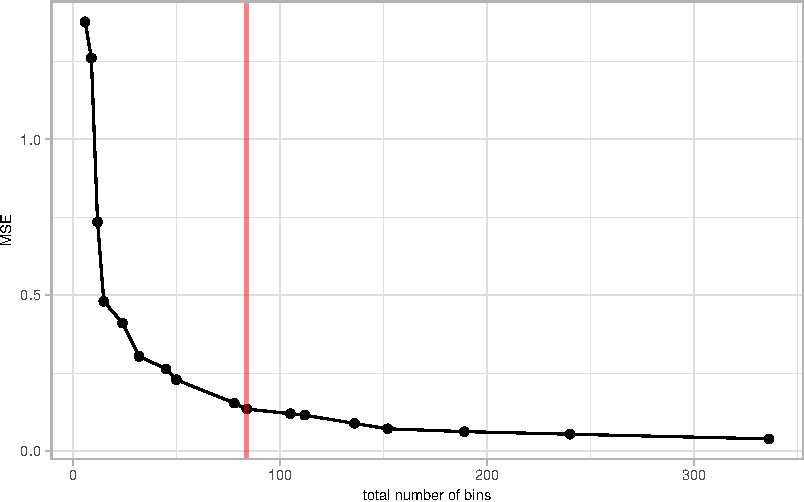
\includegraphics{paper_files/figure-pdf/fig-diagnosticpltScurve-1.pdf}

}

\caption{\label{fig-diagnosticpltScurve}Goodness of fit statistics from
UMAP applied to training S-curve dataset. What is the effective number
of bins in each NLDR technique to create a 2D model? The MSE plot have a
steep slope at the beginning, indicating that a smaller number of bins
causes a larger amount of error. Then, the slope gradually declines or
level off, indicating that a higher number of bins generates a smaller
error. Using the elbow method, when the total number of bins is set to
\(84\), the slope of the Mean Squared Error (MSE) plot experiences a
sudden and noticeable change, resembling an elbow-like shape. This point
indicates that adding less bins does not enough to capture the data
structure.}

\end{figure}

\hypertarget{benchmark-value-to-remove-low-density-hexagons}{%
\subsubsection{Benchmark value to remove low-density
hexagons}\label{benchmark-value-to-remove-low-density-hexagons}}

After setting up the hexagonal grid with an appropriate number of bins,
it is possible that some hexagonal bins may have very few or no data
points within them. To ensure comprehensive coverage of the NLDR data,
it is necessary to select hexagonal bins that have a considerable number
of data points within their hexagons. To achieve this, the number of
points within each hexagon is first calculated. Then, the standard count
is computed by dividing the number of points within each hexagon by the
maximum number of points in the grid (see Equation~\ref{eq-equationp2}).
Next, the bins that have a standard number of points less than a certain
benchmark value are removed. After removing the hexagons that have
insufficient data density, the hexagons with more substantial data
representation are used to construct the 2D model.

\begin{equation}\protect\hypertarget{eq-equationp2}{}{
\text{standard count} = \frac{\text{count}}{\text{max count}} 
}\label{eq-equationp2}\end{equation}

Furthermore, it is crucial to choose the benchmark value to remove
low-density hexagons carefully. If we remove unnecessary bins, then it
may result in long edges and an uneven 2D model. Therefore, instead of
removing hexagons only identified by the benchmark value, we examine the
standard number of points in the neighboring hexagons of the identified
low-density hexagons. If the neighboring bins also have low counts, then
only those bins will be removed. The other identified bins will be kept
and used for constructing the 2D model along with the high-density bins.

The benchmark value for removing low-density hexagons has a range of
\(0\) and \(1\). When analyzing how these benchmark values affect model
performance, it's important to observe the change in Mean Squared Error
(MSE) as the benchmark value increases. The MSE exhibits a gradual
increase as the benchmark value progresses from \(0\) to \(1\).
Assessing this rate of increase is crucial. If the increment is not
substantial, the decision might lean towards retaining low-density
hexagons.

The following steps will help to find a suitable value to remove low
density hexagons:

\begin{enumerate}
\def\labelenumi{\arabic{enumi}.}
\tightlist
\item
  Plot the distribution of the standardized counts
\end{enumerate}

\begin{figure}[H]

{\centering 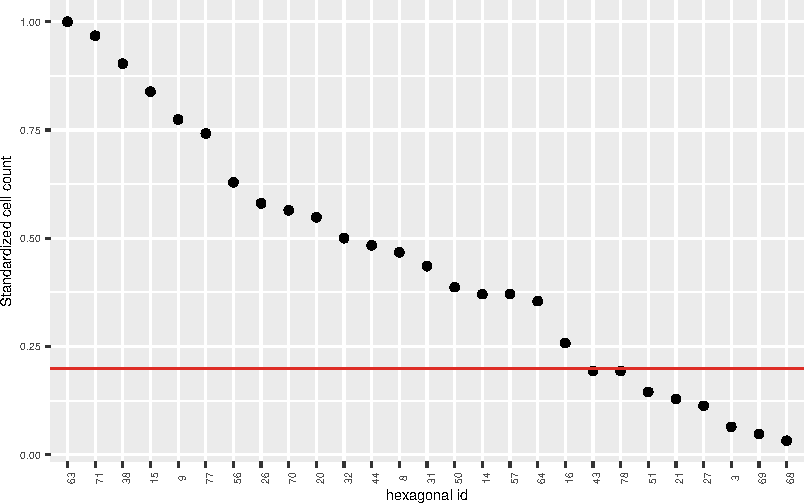
\includegraphics{paper_files/figure-pdf/fig-stdctsScurve-1.pdf}

}

\caption{\label{fig-stdctsScurve}Distribution of 2D Euclidean
distances.}

\end{figure}

\begin{enumerate}
\def\labelenumi{\arabic{enumi}.}
\setcounter{enumi}{1}
\item
  See the distribution of counts
\item
  Take the first quartile
\end{enumerate}

\begin{figure}

{\centering 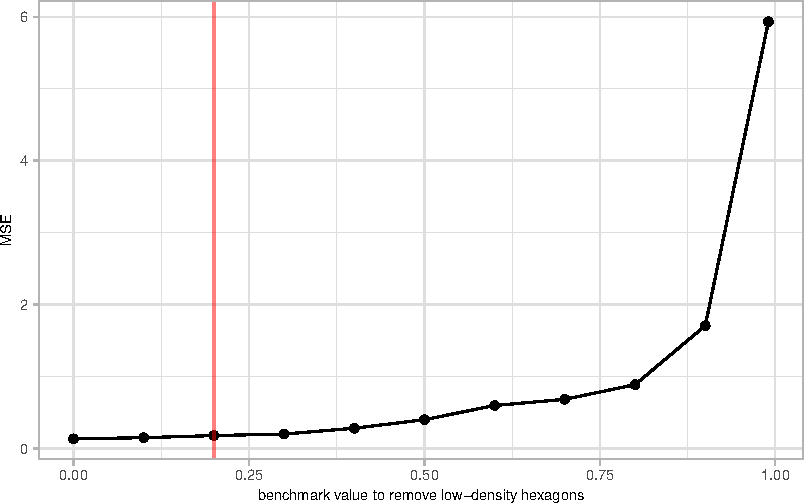
\includegraphics{paper_files/figure-pdf/fig-diagnosticpltScurvelwd-1.pdf}

}

\caption{\label{fig-diagnosticpltScurvelwd}Goodness of fit statistics
from UMAP applied to training S-curve dataset with different benchmark
values to remove the low-density heaxgons. What is the effective
benchmark value to remove the low-density heaxgons? The MSE plot have a
steep slope at the beginning, indicating that a smaller benchmark causes
a small amount of error. Then, the slope gradually increases or level
up, indicating that a higher number of benchmark values generates a
higher error. Using the reverse elbow method, when the benchmark value
is set to 0.2, the slope of the Mean Squared Error (MSE) plot
experiences a sudden and noticeable change, resembling an elbow-like
shape. This point indicates that higher benchmark values remove the
necessary bins as well which lead to distruct the 2D structure.}

\end{figure}

\begin{figure}[H]

{\centering 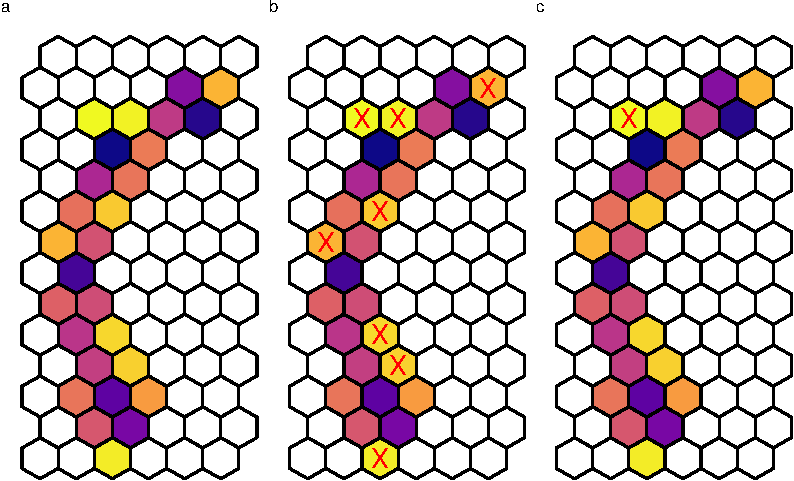
\includegraphics{paper_files/figure-pdf/fig-rmlowdenshex-1.pdf}

}

\caption{\label{fig-rmlowdenshex}Goodness of f}

\end{figure}

\hypertarget{benchmark-value-to-remove-long-edges}{%
\subsubsection{Benchmark value to remove long
edges}\label{benchmark-value-to-remove-long-edges}}

Achieving a smooth representation in 2D space is crucial, and one factor
influencing this smoothness is the presence of long edges (see
\textbf{?@fig-modelScurvermlgimp}). These long edges occur when a line
connects points that are distant in the triangular mesh, impacting the
overall smoothness of the mesh.

To investigate the effect of removing long edges on the MSE, we analyzed
the MSE for various benchmark values. Surprisingly, the results
indicated that the MSE remained consistent across different benchmark
values, as shown in \textbf{?@fig-diagnosticpltScurvelgrm}. It's
important to note that edges are defined only in the 2D model and do not
extend to higher dimensions. Consequently, removing edges does not
affect the model in higher dimensions.

There is no definitive rule for determining the benchmark value to
remove long edges. However, we have a method to find a default value
(see Appendix). Adjusting values around this default can help to find
benchmark value to remove long edges, contributing to the construction
of a smoother 2D representation (see
\textbf{?@fig-diagnosticpltScurvelgrm}).

The following steps will help to find a suitable value to remove long
edges:

\begin{enumerate}
\def\labelenumi{\arabic{enumi}.}
\tightlist
\item
  Plot the distribution of the 2D distances
\end{enumerate}

\begin{figure}[H]

{\centering 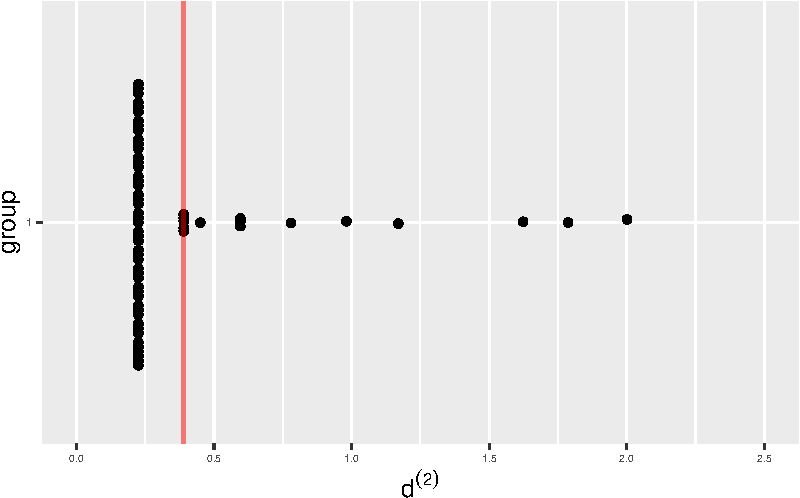
\includegraphics{paper_files/figure-pdf/fig-distScurve-1.pdf}

}

\caption{\label{fig-distScurve}Distribution of 2D Euclidean distances.}

\end{figure}

\begin{enumerate}
\def\labelenumi{\arabic{enumi}.}
\setcounter{enumi}{1}
\tightlist
\item
  Find a value which is greater than smallest value
\end{enumerate}

\begin{figure}[H]

{\centering 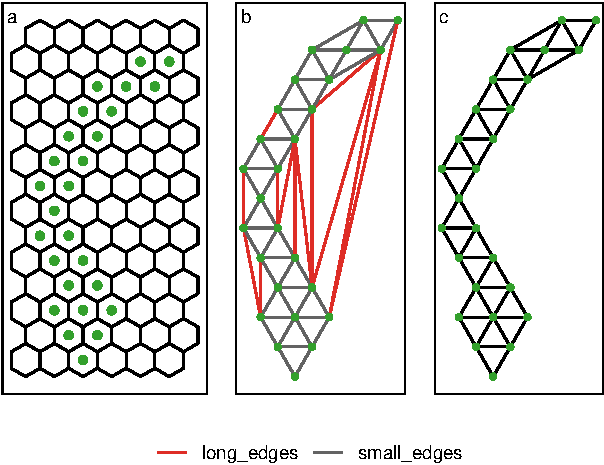
\includegraphics{paper_files/figure-pdf/fig-modelScurve-1.pdf}

}

\caption{\label{fig-modelScurve}(a) Full hexagonal grid with bin
centroids, (b) Model constructed in 2D with long edges, and (c) Model
constructed in 2D after removing the long edges.}

\end{figure}

\hypertarget{starting-point-of-the-hexagonal-grid}{%
\subsubsection{Starting point of the hexagonal
grid}\label{starting-point-of-the-hexagonal-grid}}

According to \citet{Dan2023}, the hexagonal binning is done by
tessellating the \(xy\) plane over the set (range(\(x\)), range(\(y\)))
(see Figure~\ref{fig-scurveshifthexgridsexp} (b)). In that case, bin
centroids are defined as shown in
Figure~\ref{fig-scurveshifthexgridsexp} (a) with gray colour. Rather
than sticking to the typical hexagonal grid, introducing a meaningful
shift in both the x and y directions presents an opportunity for an
improved 2D model. Therefore, investigating this shift in the hexagonal
grid is an important parameter to consider.

As shown in Figure~\ref{fig-scurveshifthexgrids}, the shifting
influences the distribution of points and number of non-empty bins,
impacting the resulting 2D model. According to
\textbf{?@fig-diagnosticpltScurvehexbins}, the 2D model with a total of
\(144\) bins applied to S-curve UMAP data does not require any shifting
because the lowest MSE occurs when no shift is introduced.

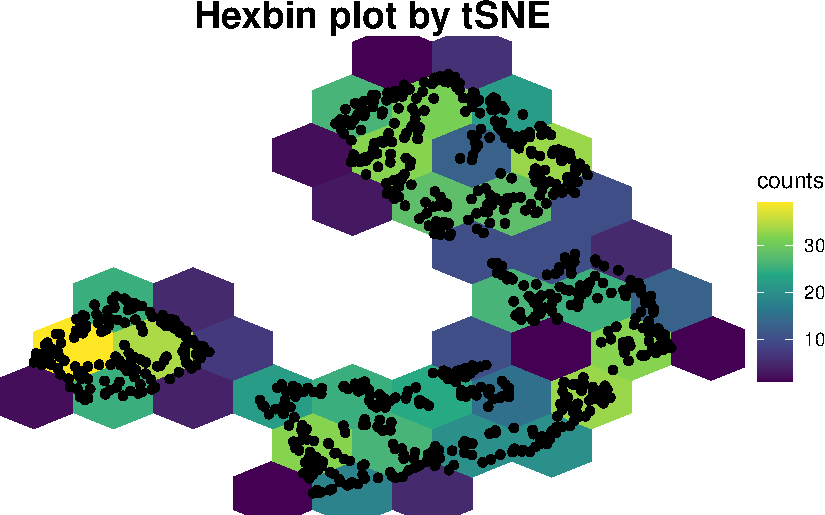
\includegraphics{paper_files/figure-pdf/unnamed-chunk-36-1.pdf}

\begin{figure}

{\centering 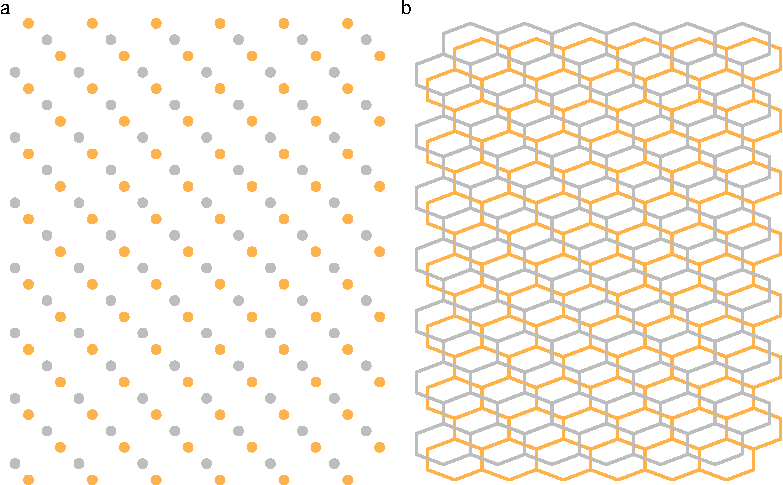
\includegraphics{paper_files/figure-pdf/fig-scurveshifthexgridsexp-1.pdf}

}

\caption{\label{fig-scurveshifthexgridsexp}(a) Visualization of bin
centroids and (b) hexagonal grid, showcasing the configuration before
(colored in gray) and after (colored in light orange) shifting the
starting point by an identical amount applied in both x and y
directions, with a shift value of \(0.537285\).}

\end{figure}

\begin{figure}

{\centering 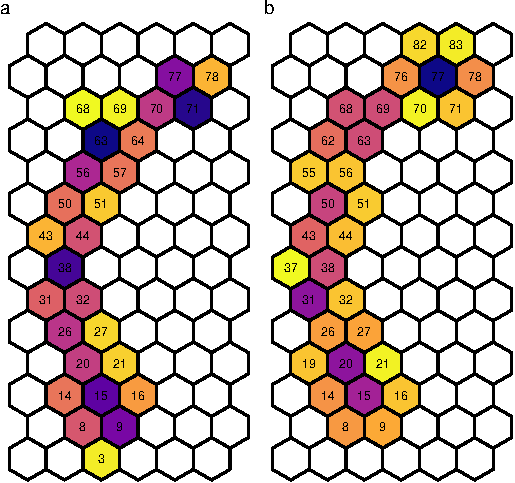
\includegraphics{paper_files/figure-pdf/fig-scurveshifthexgrids-1.pdf}

}

\caption{\label{fig-scurveshifthexgrids}Hexbin plots shows the
distribution of points before and after shifting the starting point of
the hexagonal grid generated for UMAP applied to the training S-curve
dataset. (a) Hexbin plot before shifting, and (b) Hexbin plot after
shifting (identical shift applied in both x and y directions, with a
shift value of \(0.537285\)).}

\end{figure}

\hypertarget{sec-summary}{%
\subsection{Model summaries}\label{sec-summary}}

\hypertarget{predicted-values-and-residuals}{%
\subsubsection{Predicted values and
residuals}\label{predicted-values-and-residuals}}

The prediction approach involves performing the K-nearest neighbors
(KNN) algorithm for an unsupervised classification problem. First, the
nearest high-D model point is identified for a given new high-D point.
Then, the corresponding 2D centroid mapping for the identified high-D
model point is determined. Finally, the coordinates of this 2D centroid
are used as the predicted 2D embedding for the new high-D data point.
This step is particularly valuable due to the limitations of some NLDR
techniques, like tSNE, which don't provide a straightforward method for
prediction. As a result, our approach offers a solution that capable of
generating predicted 2D embedding regardless of the NLDR technique
employed, effectively addressing this functional gap.

Residuals are essential for evaluating the accuracy of representing
high-D points by the high-D mapping of 2D bin centroids. To measure this
accuracy, an error metric is introduced, quantifying the sum of squared
differences between the high-D data (\(x_{ij}\)) and the high-D mapping
of the 2D bin centroid data (\(C_{x_ij}\)) across all observations and
dimensions (see Equation~\ref{eq-equation10}).

\begin{equation}\protect\hypertarget{eq-equation10}{}{
\text{Error} = \sum_{j = 1}^{n}\sum_{i = 1}^{p} (x_{ij} - C_{x_ij})^2
}\label{eq-equation10}\end{equation}

Here, \(n\) represents the number of observations, \(p\) represents the
dimensions of high-D data, \(x_{ij}\) is the high-D data, and
\(C_{x_ij}\) is the high-D mapping of the 2D bin centroid.

\hypertarget{sec-goodfit}{%
\subsubsection{Goodness of fit statistics}\label{sec-goodfit}}

To assess how well our method captures and represents the underlying
structure of the high-D data, Mean Squared Error (MSE) is used. When
computing MSE, total model error (see Section~\ref{sec-summary}) is
divided by the number of observations to make it as a mean value (see
Equation~\ref{eq-equation9}).

\begin{equation}\protect\hypertarget{eq-equation9}{}{
\text{MSE} = \sum_{j = 1}^{n} \frac{\sum_{i = 1}^{p} (x_{ij} - C_{x_ij})^2}{n}
}\label{eq-equation9}\end{equation}

\hypertarget{sec-simpleex}{%
\subsection{Simulated data example}\label{sec-simpleex}}

In this section, we showcase the effectiveness of our methodology using
simulated data. The dataset comprises five spherical Gaussian clusters
in 4-\(d\), with each cluster containing an equal number of points and
consistent within variation.

In the 2D representations created by all NLDR techniques, as shown in
Figure~\ref{fig-nldervis5Gau}, except for PHATE, there are five distinct
clusters. In tSNE, these five clusters are closely located to each other
(see Figure~\ref{fig-nldervis5Gau} (a)). However, in PHATE, two clusters
are closely positioned, while the other three are more distant (see
Figure~\ref{fig-nldervis5Gau} (c)). In PaCMAP, one cluster is at the
center, and the remaining four are positioned in four different
directions (see Figure~\ref{fig-nldervis5Gau} (e)). In TriMAP, two
clusters are close, although not as close as in PHATE, and the other
three are well-separated (see Figure~\ref{fig-nldervis5Gau} (d)). In
UMAP, all clusters are arranged in a parallel manner, with three in one
line and the other two in a separate line (see
Figure~\ref{fig-nldervis5Gau} (b)).

Visualizing the models alongside the original high-D data provides
insights into how different techniques capture the underlying clustering
structure. The tSNE model exhibits five well-separated clusters,
effectively preserving both local and global structures (see video link
of Figure~\ref{fig-modelfiveGau} (a)). UMAP, on the other hand, also
presents five distinct clusters but with a more flattened surface
appearance (see video link of Figure~\ref{fig-modelfiveGau} (b)). The
PHATE model shows five separated clusters resembling triangles or
partial triangles but struggles to capture local structures (see video
link of Figure~\ref{fig-modelfiveGau} (c)). TriMAP and PaCMAP both
display five well-separated clusters with flat surfaces, each capturing
within-cluster variation to varying extents. Despite the various 2D
representations, all NLDR techniques preserve the global structure (see
video link of Figure~\ref{fig-modelfiveGau} (d), (e) respectively).
However, tSNE, effectively capture both local and global structures.

\begin{figure}

{\centering 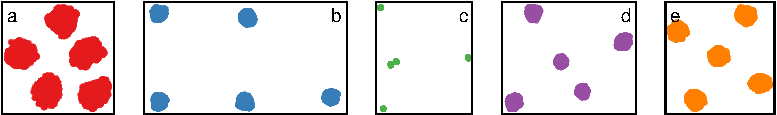
\includegraphics[width=1\textwidth,height=\textheight]{paper_files/figure-pdf/fig-nldervis5Gau-1.pdf}

}

\caption{\label{fig-nldervis5Gau}2D layouts from different NLDR
techniques applied the same data: (a) tSNE (perplexity = 61), (b) UMAP
(n\_neighbors = 15), (c) PHATE (knn = 5), (d) TriMAP (n\_inliers = 5,
n\_outliers = 4, n\_random = 3), and (e) PaCMAP (n\_neighbors = 10, init
= random, MN\_ratio = 0.9, FP\_ratio = 2). Is there a best
representation of the original data or are they all providing equivalent
information?}

\end{figure}

\begin{figure}

{\centering 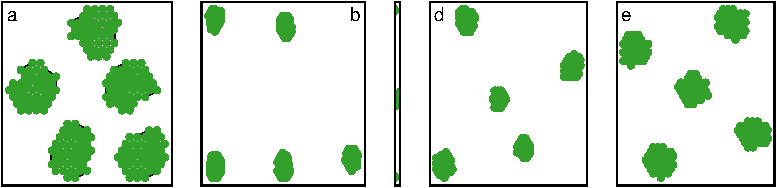
\includegraphics[width=1\textwidth,height=\textheight]{paper_files/figure-pdf/fig-modelfiveGau-1.pdf}

}

\caption{\label{fig-modelfiveGau}Is there a best model to represent the
original data in 2D space or are they all providing equivalent
information?, (a) Model generated with 21 and 28 bins along the x and y
axes, respectively, using a hexagonal size of 0.03 in the 2D space with
tSNE, (b) Model generated with 60 and 79 bins along the x and y axes,
respectively, using a hexagonal size of 0.01 in the 2D space with UMAP,
(c) Model generated with 60 and 1927 bins along the x and y axes,
respectively, using a hexagonal size of 0.01 in the 2D space with PHATE,
(d) Model generated with 46 and 61 bins along the x and y axes,
respectively, using a hexagonal size of 0.013 in the 2D space with
TriMAP, and (e) Model generated with 31 and 40 bins along the x and y
axes, respectively, using a hexagonal size of 0.02 in the 2D space with
PaCMAP.}

\end{figure}

\begin{figure}[H]

\begin{minipage}[t]{0.33\linewidth}

{\centering 

\raisebox{-\height}{

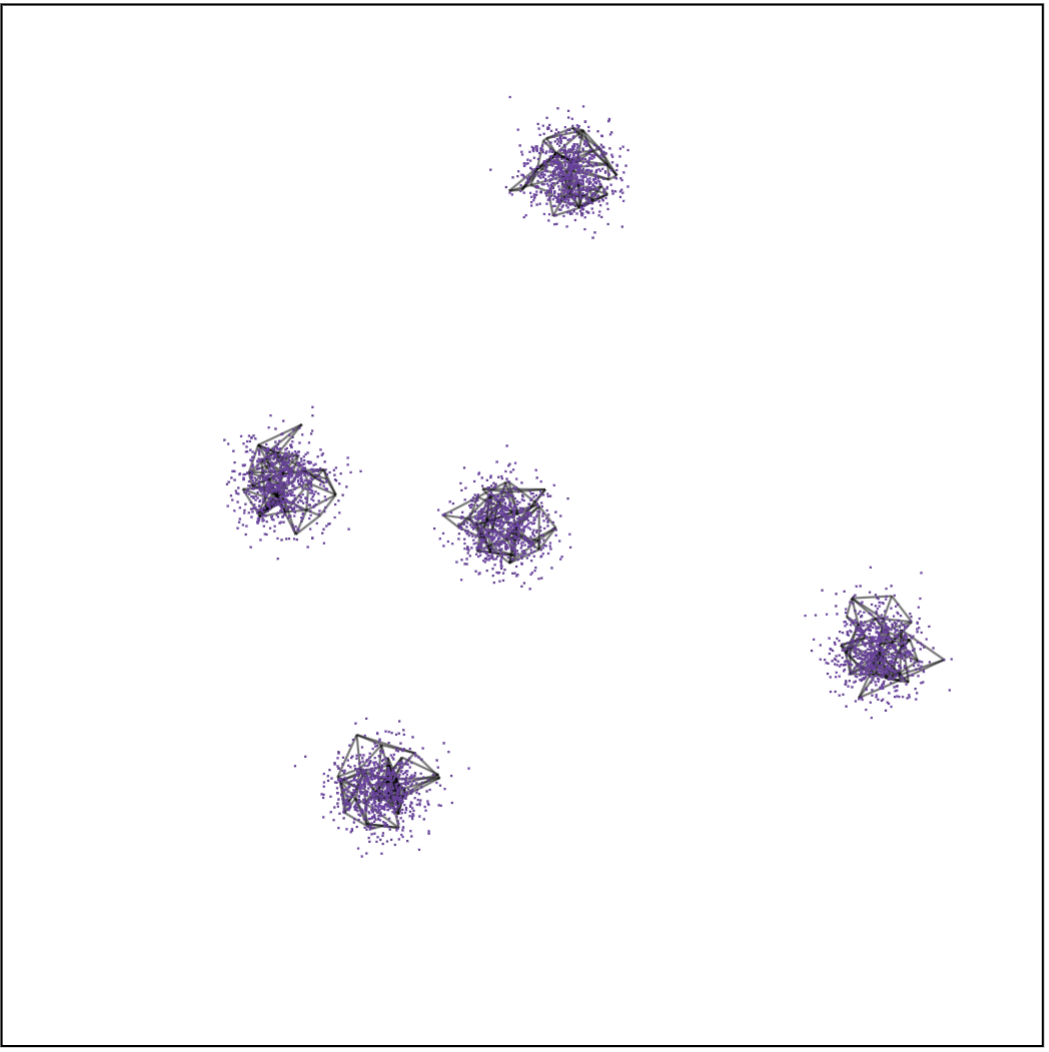
\includegraphics{figures/five_gau_clusters/sc_tsne_1.png}

}

}

\subcaption{\label{fig-gau1_sc1}}
\end{minipage}%
%
\begin{minipage}[t]{0.33\linewidth}

{\centering 

\raisebox{-\height}{

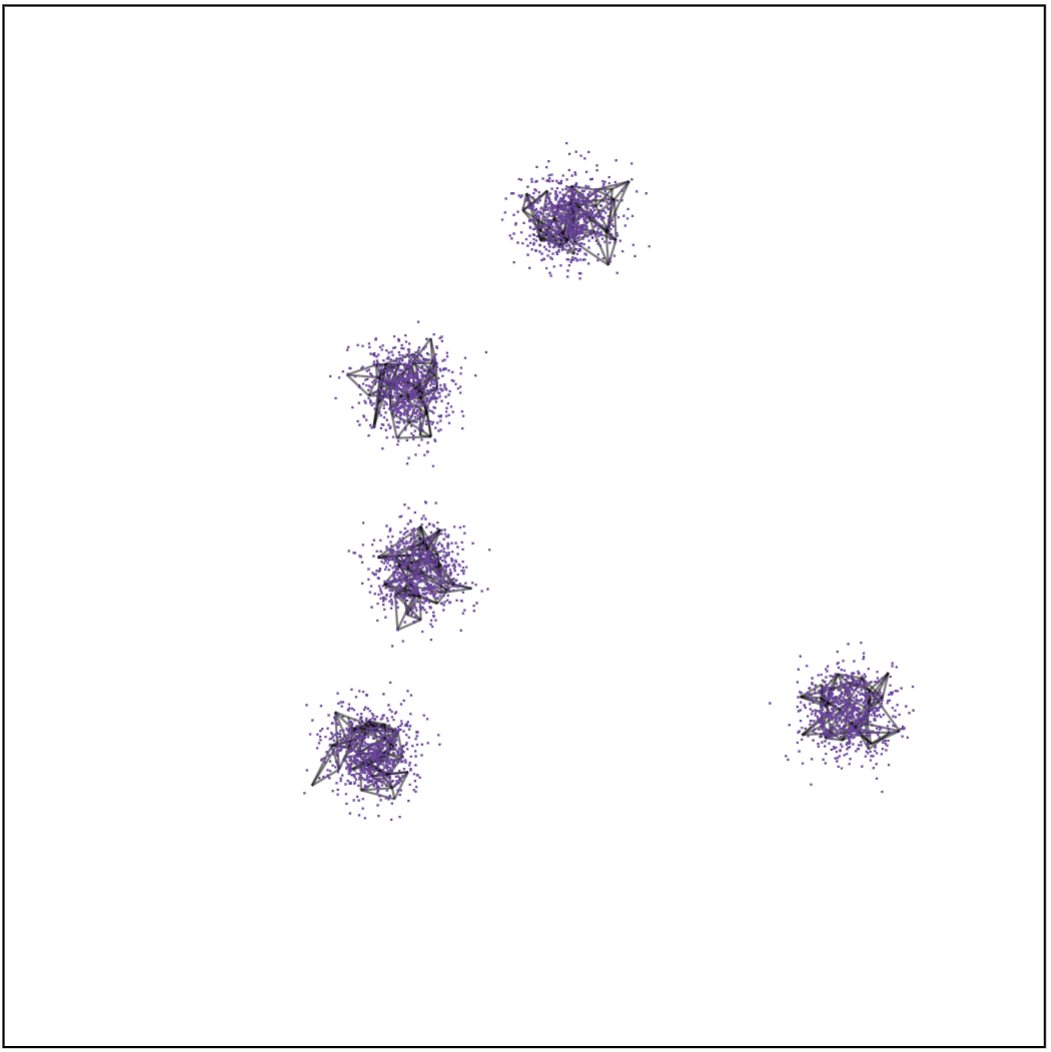
\includegraphics{figures/five_gau_clusters/sc_tsne_2.png}

}

}

\subcaption{\label{fig-gau1_sc2}}
\end{minipage}%
%
\begin{minipage}[t]{0.33\linewidth}

{\centering 

\raisebox{-\height}{

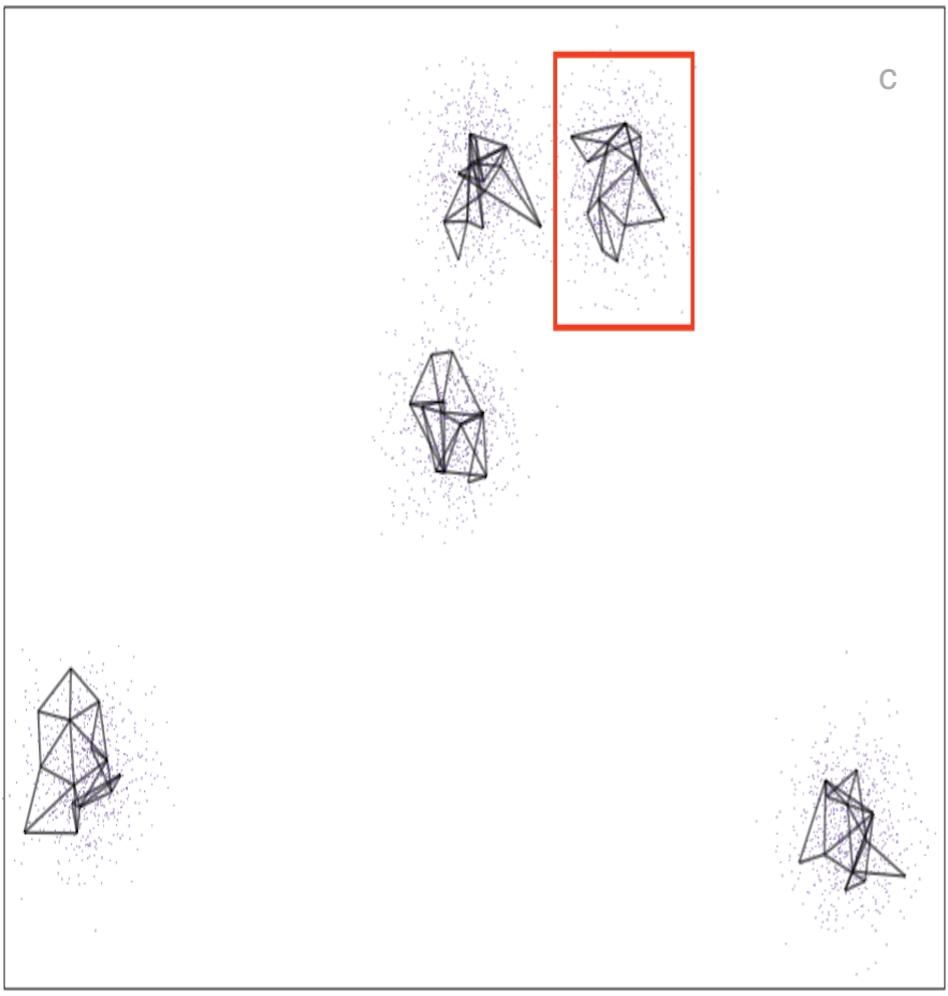
\includegraphics{figures/five_gau_clusters/sc_tsne_3.png}

}

}

\subcaption{\label{fig-gau1_sc3}}
\end{minipage}%

\caption{\label{fig-gau1_sc}Screen shots of the \textbf{langevitour} of
the five Gaussian clusters dataset, shows the model with tSNE in high-D,
a video of the tour animation is available at
(\url{https://youtu.be/oQxEb4wRdHI}).}

\end{figure}

\begin{figure}[H]

\begin{minipage}[t]{0.33\linewidth}

{\centering 

\raisebox{-\height}{

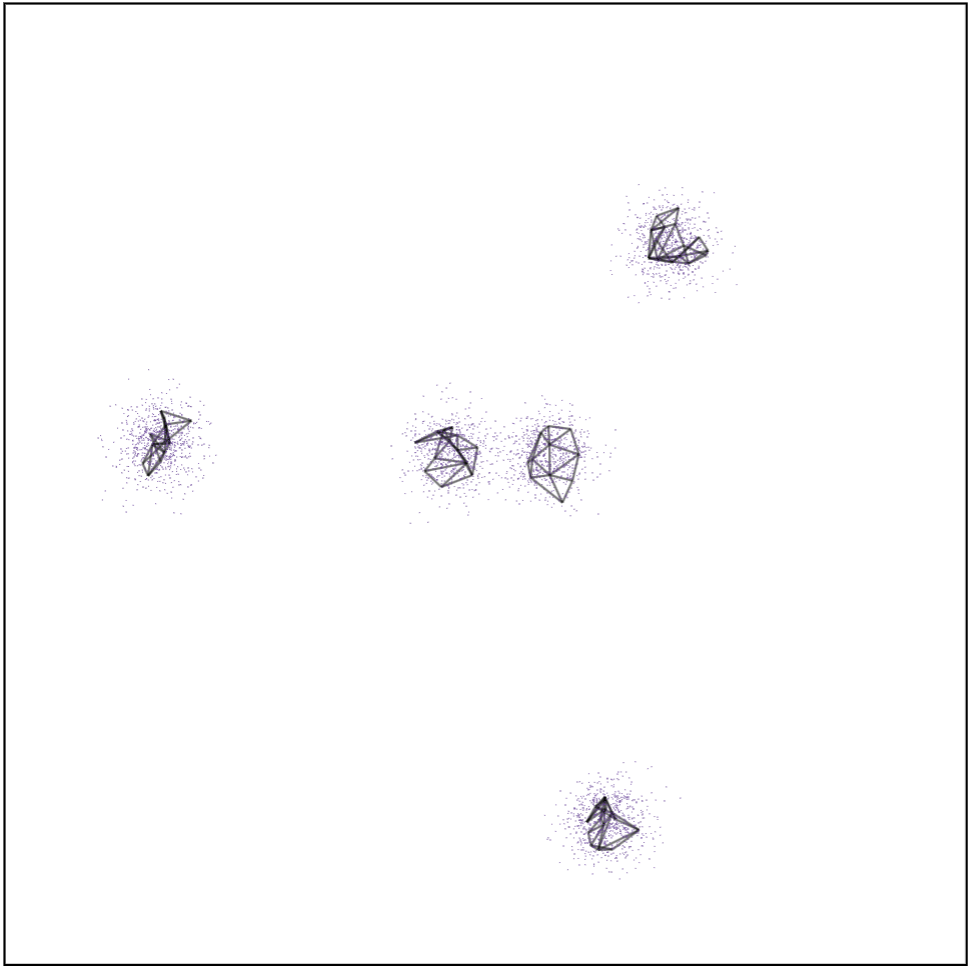
\includegraphics{figures/five_gau_clusters/sc_umap_1.png}

}

}

\subcaption{\label{fig-gau2_sc1}}
\end{minipage}%
%
\begin{minipage}[t]{0.33\linewidth}

{\centering 

\raisebox{-\height}{

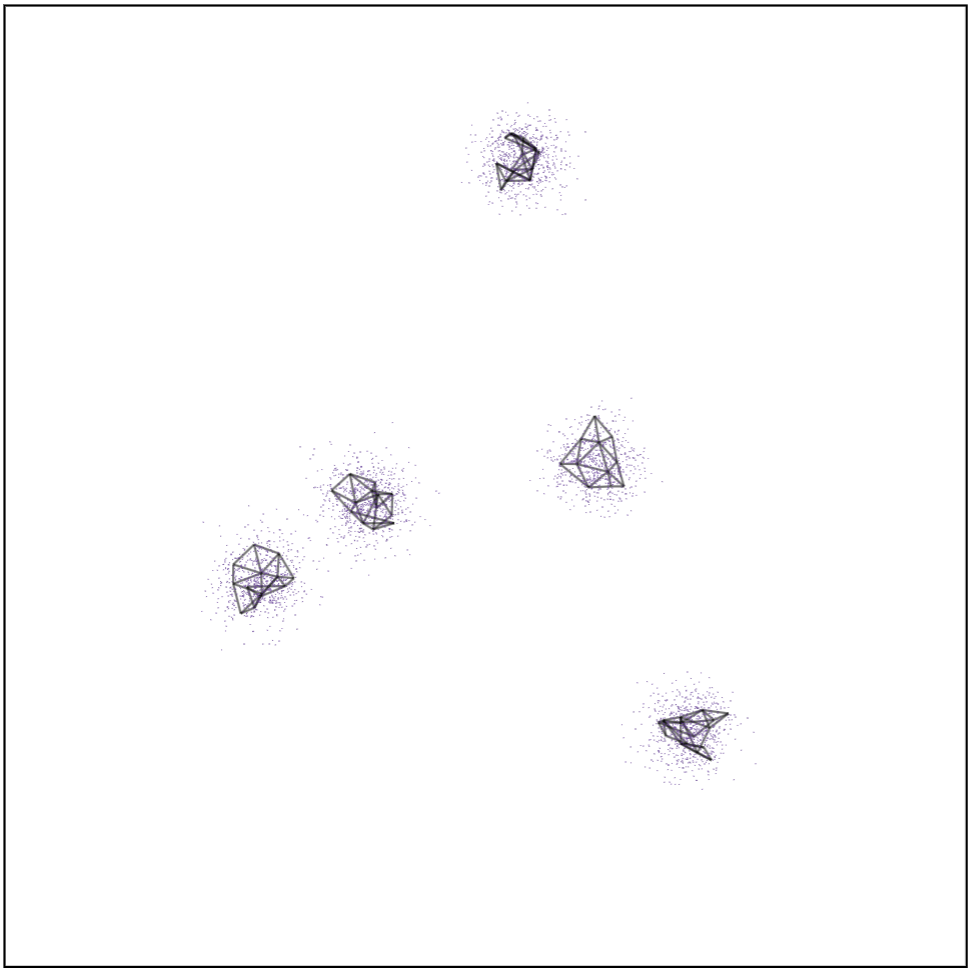
\includegraphics{figures/five_gau_clusters/sc_umap_2.png}

}

}

\subcaption{\label{fig-gau2_sc2}}
\end{minipage}%
%
\begin{minipage}[t]{0.33\linewidth}

{\centering 

\raisebox{-\height}{

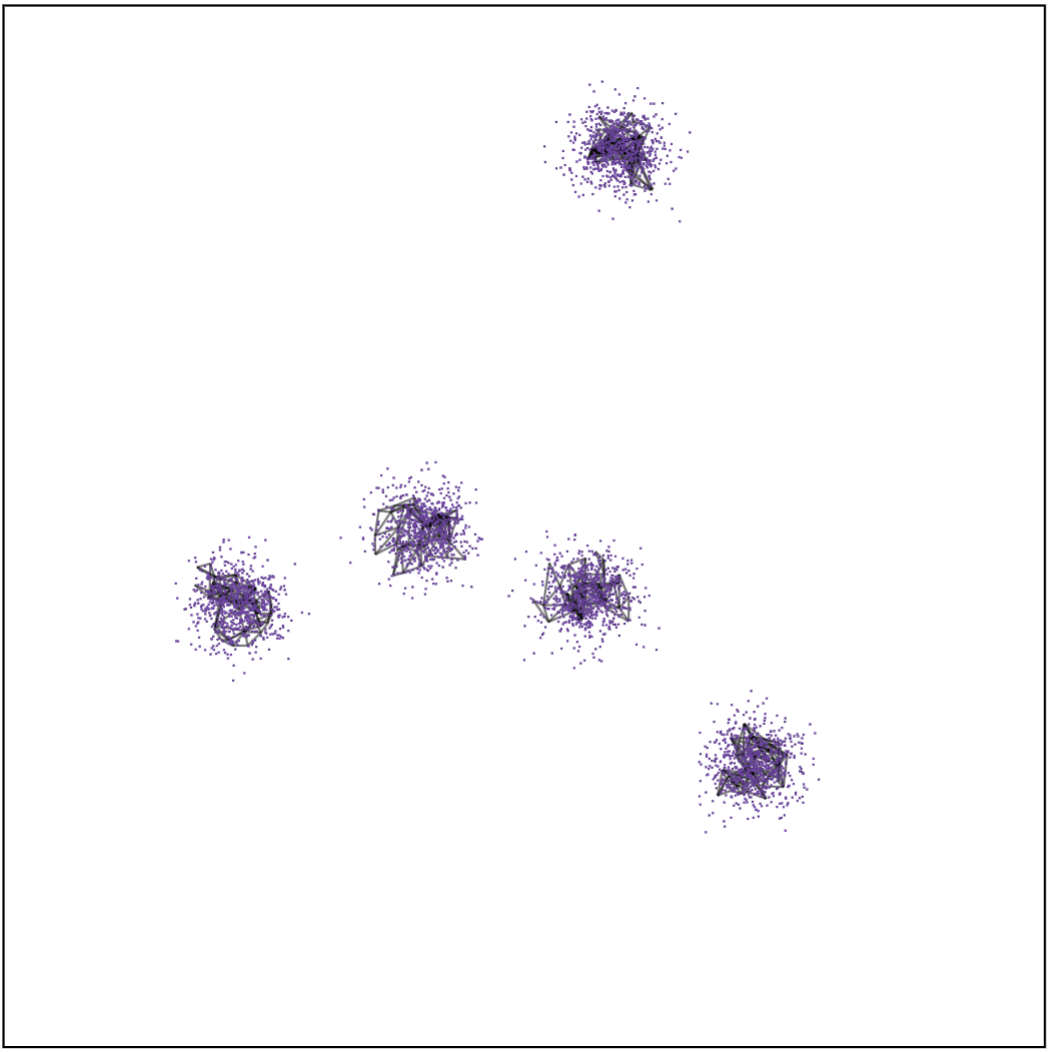
\includegraphics{figures/five_gau_clusters/sc_umap_3.png}

}

}

\subcaption{\label{fig-gau2_sc3}}
\end{minipage}%

\caption{\label{fig-gau2_sc}Screen shots of the \textbf{langevitour} of
the five Gaussian clusters dataset, shows the model with UMAP in high-D,
a video of the tour animation is available at
(\url{https://youtu.be/JW49csPpDx4}).}

\end{figure}

\begin{figure}[H]

\begin{minipage}[t]{0.33\linewidth}

{\centering 

\raisebox{-\height}{

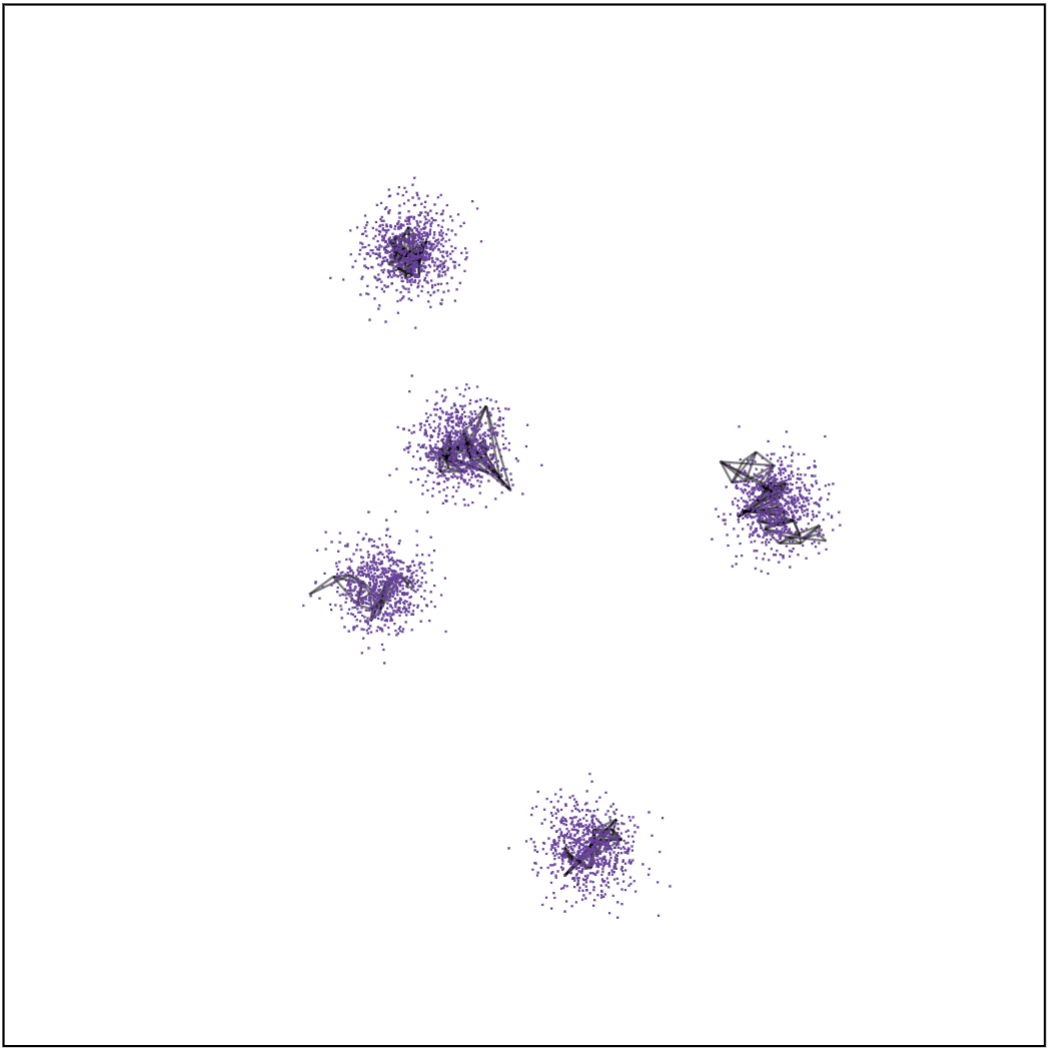
\includegraphics{figures/five_gau_clusters/sc_phate_1.png}

}

}

\subcaption{\label{fig-gau3_sc1}}
\end{minipage}%
%
\begin{minipage}[t]{0.33\linewidth}

{\centering 

\raisebox{-\height}{

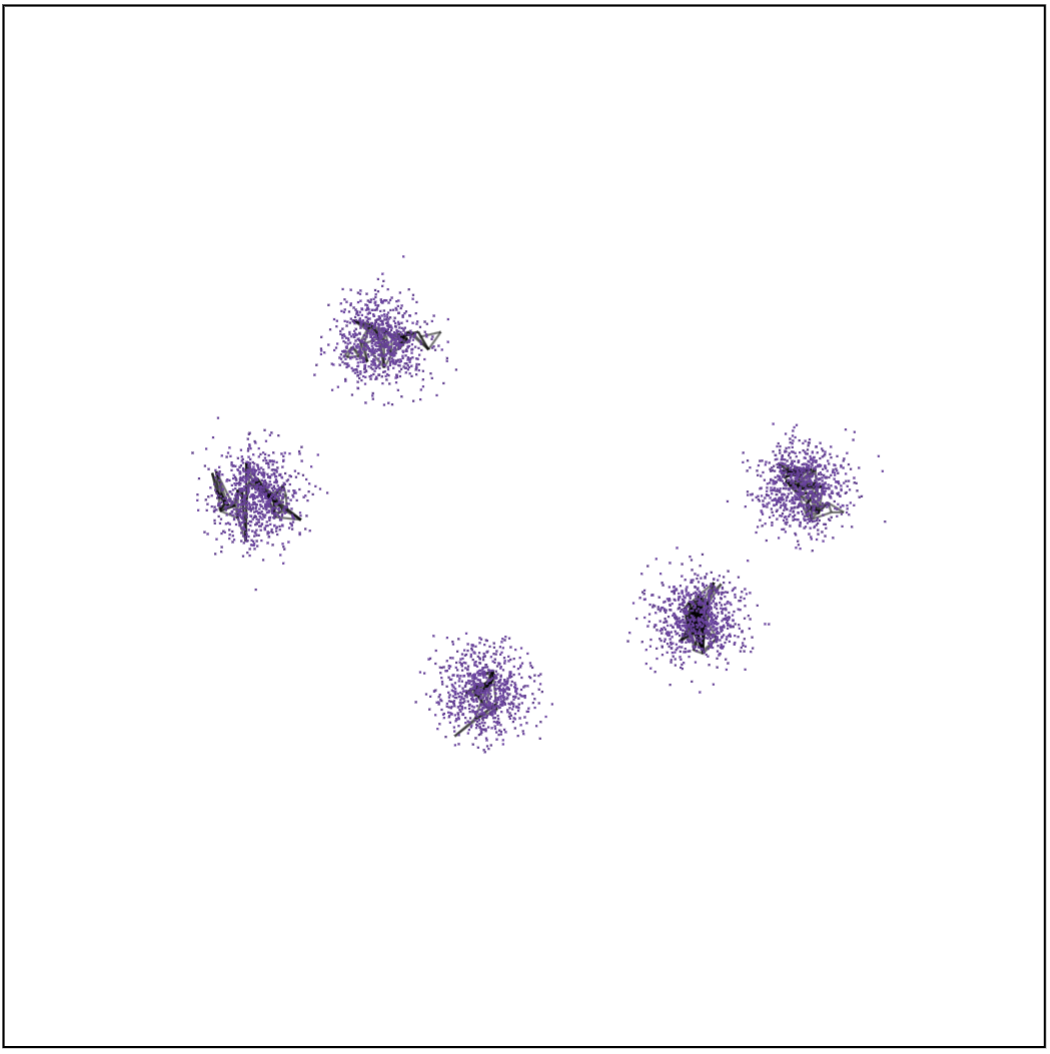
\includegraphics{figures/five_gau_clusters/sc_phate_2.png}

}

}

\subcaption{\label{fig-gau3_sc2}}
\end{minipage}%
%
\begin{minipage}[t]{0.33\linewidth}

{\centering 

\raisebox{-\height}{

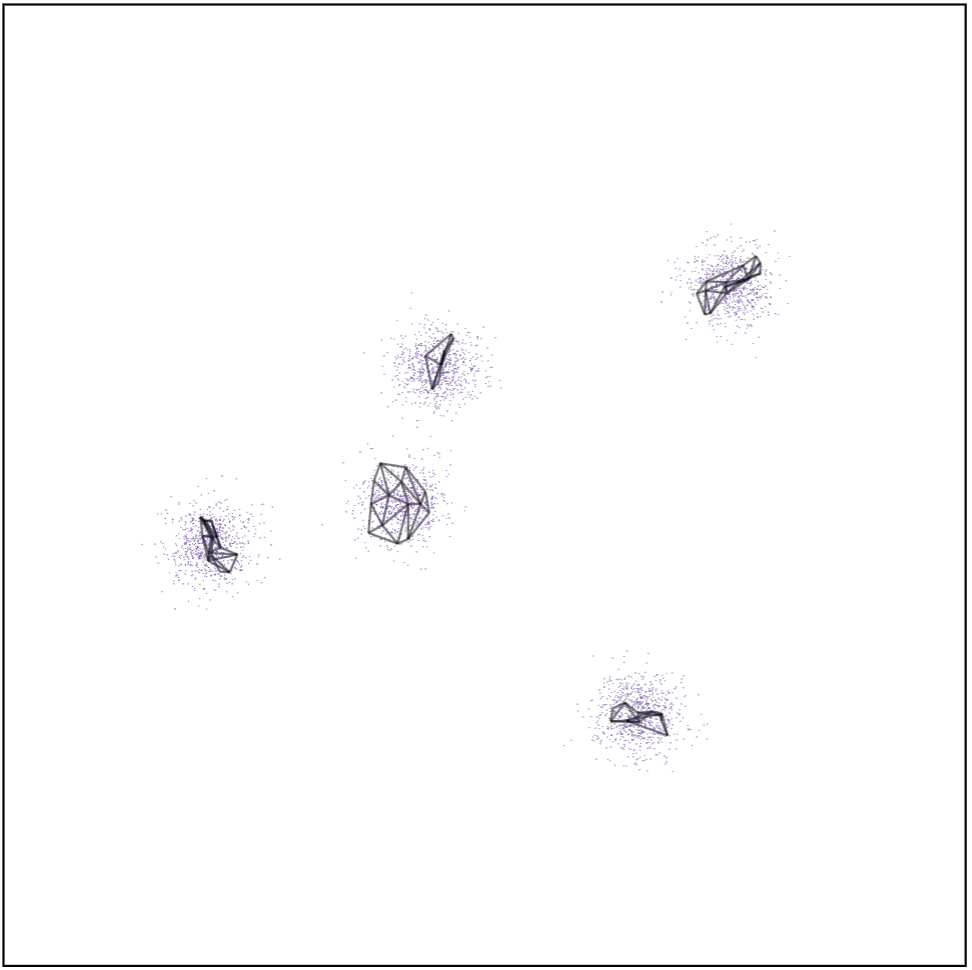
\includegraphics{figures/five_gau_clusters/sc_phate_3.png}

}

}

\subcaption{\label{fig-gau3_sc3}}
\end{minipage}%

\caption{\label{fig-gau3_sc}Screen shots of the \textbf{langevitour} of
the five Gaussian clusters dataset, shows the model with PHATE in
high-D, a video of the tour animation is available at
(\url{https://youtu.be/xqhRODt8Z-o}).}

\end{figure}

\begin{figure}[H]

\begin{minipage}[t]{0.33\linewidth}

{\centering 

\raisebox{-\height}{

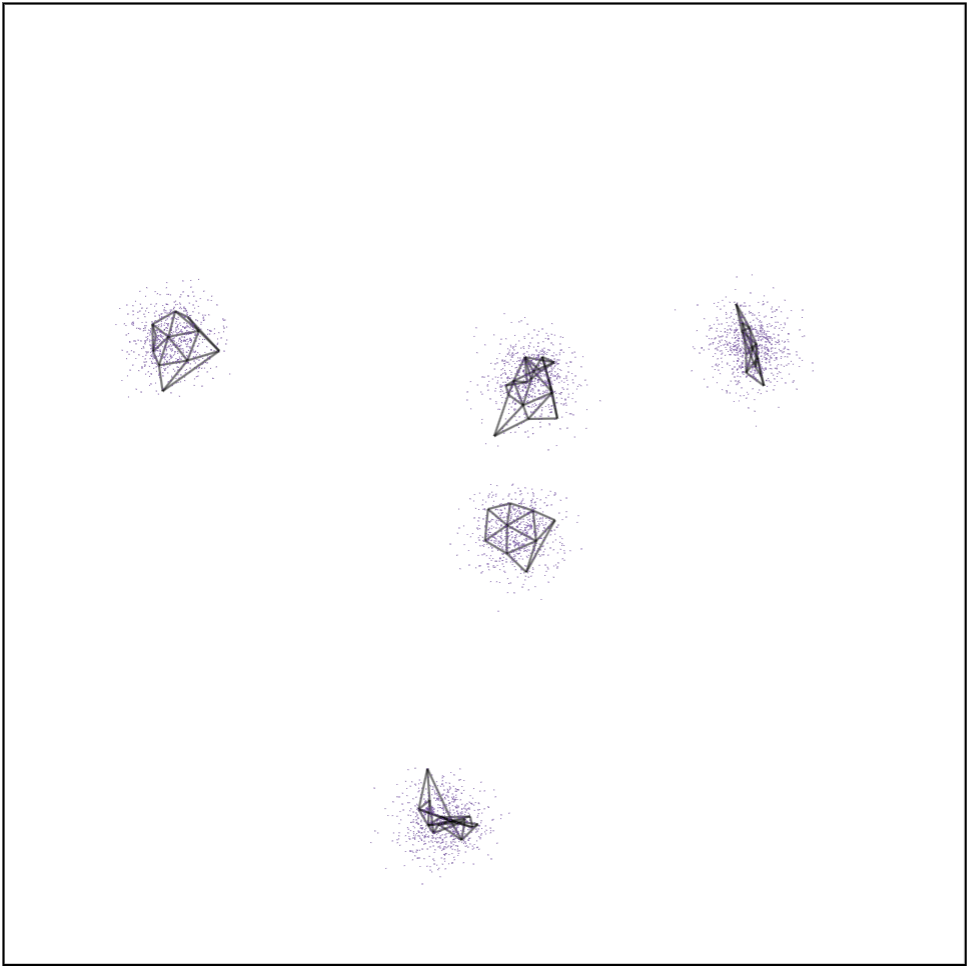
\includegraphics{figures/five_gau_clusters/sc_trimap_1.png}

}

}

\subcaption{\label{fig-gau4_sc1}}
\end{minipage}%
%
\begin{minipage}[t]{0.33\linewidth}

{\centering 

\raisebox{-\height}{

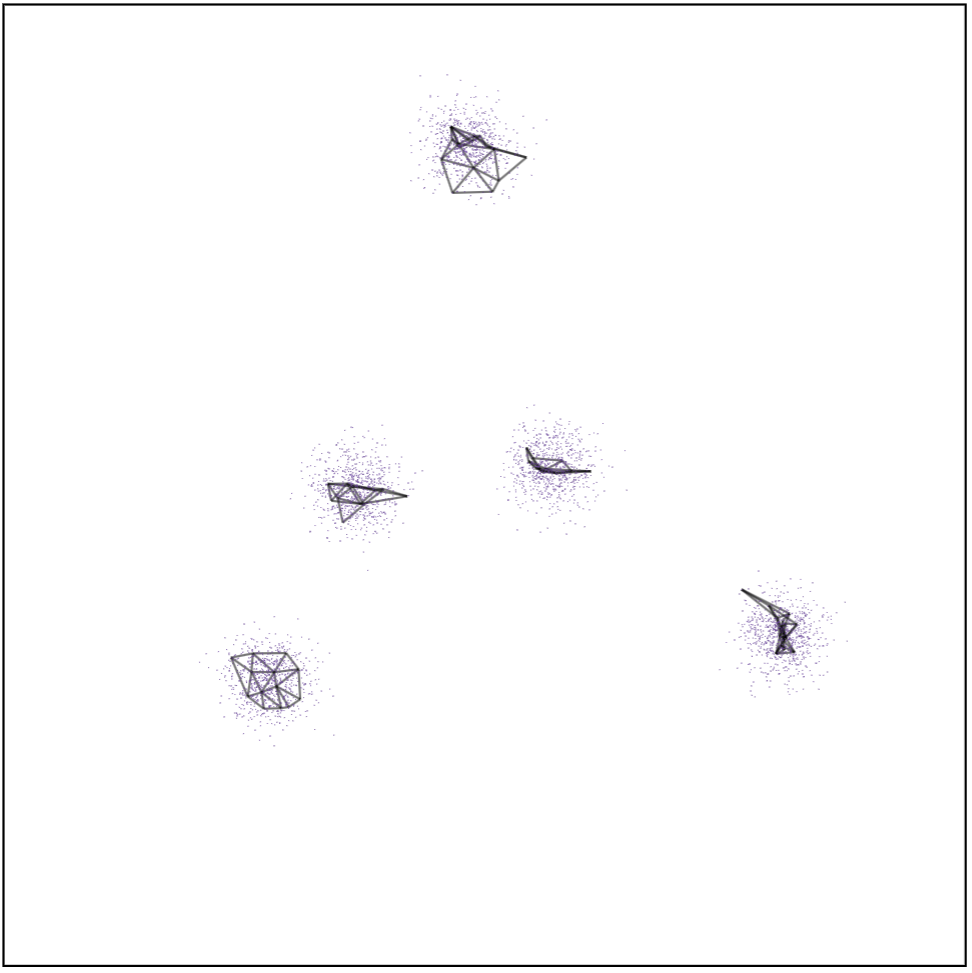
\includegraphics{figures/five_gau_clusters/sc_trimap_2.png}

}

}

\subcaption{\label{fig-gau4_sc2}}
\end{minipage}%
%
\begin{minipage}[t]{0.33\linewidth}

{\centering 

\raisebox{-\height}{

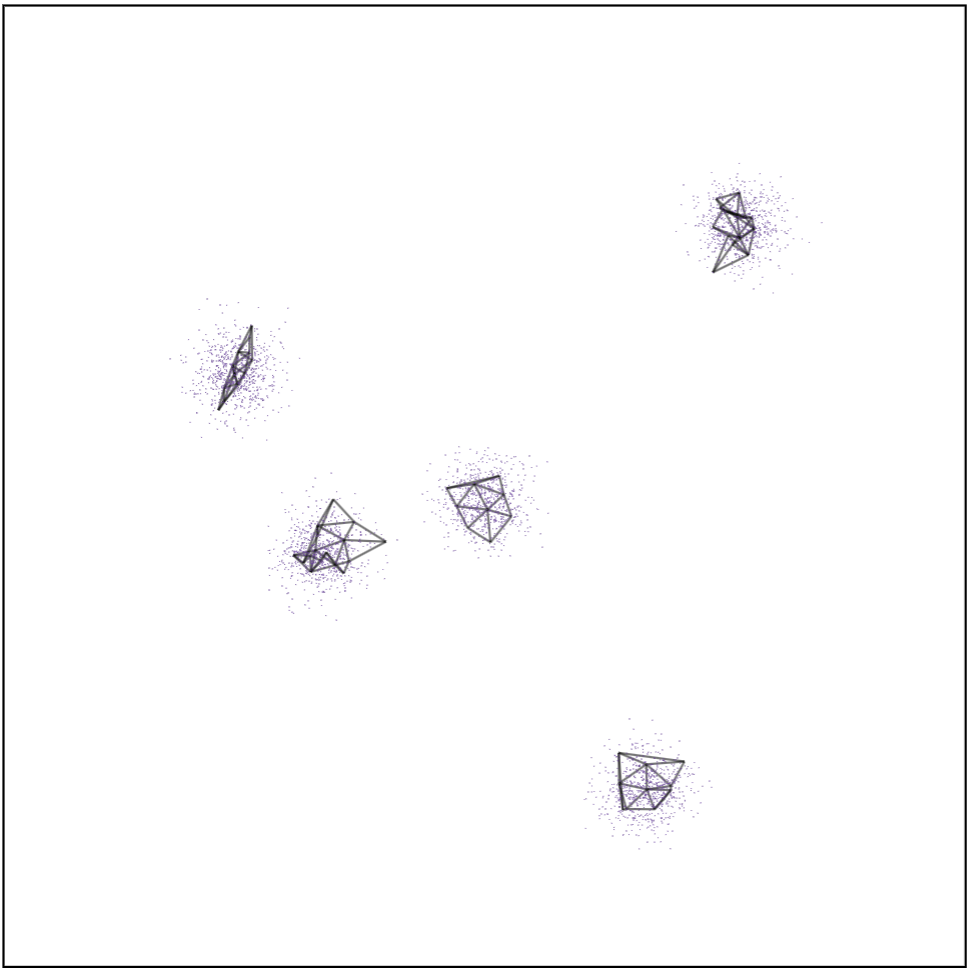
\includegraphics{figures/five_gau_clusters/sc_trimap_3.png}

}

}

\subcaption{\label{fig-gau4_sc3}}
\end{minipage}%

\caption{\label{fig-gau4_sc}Screen shots of the \textbf{langevitour} of
the five Gaussian clusters dataset, shows the model with TriMAP in
high-D, a video of the tour animation is available at
(\url{https://youtu.be/X-uHSB4VoZ0}).}

\end{figure}

\begin{figure}[H]

\begin{minipage}[t]{0.33\linewidth}

{\centering 

\raisebox{-\height}{

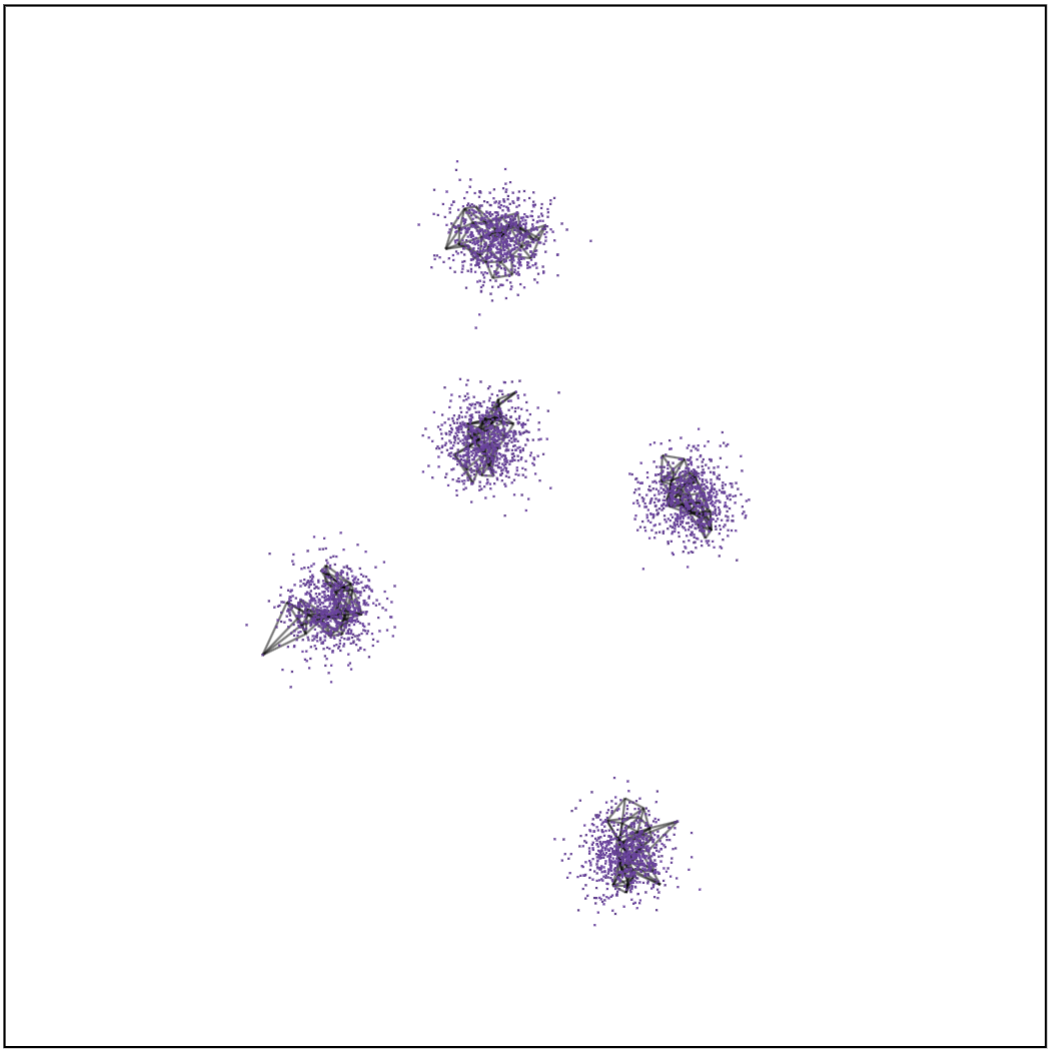
\includegraphics{figures/five_gau_clusters/sc_pacmap_1.png}

}

}

\subcaption{\label{fig-gau5_sc1}}
\end{minipage}%
%
\begin{minipage}[t]{0.33\linewidth}

{\centering 

\raisebox{-\height}{

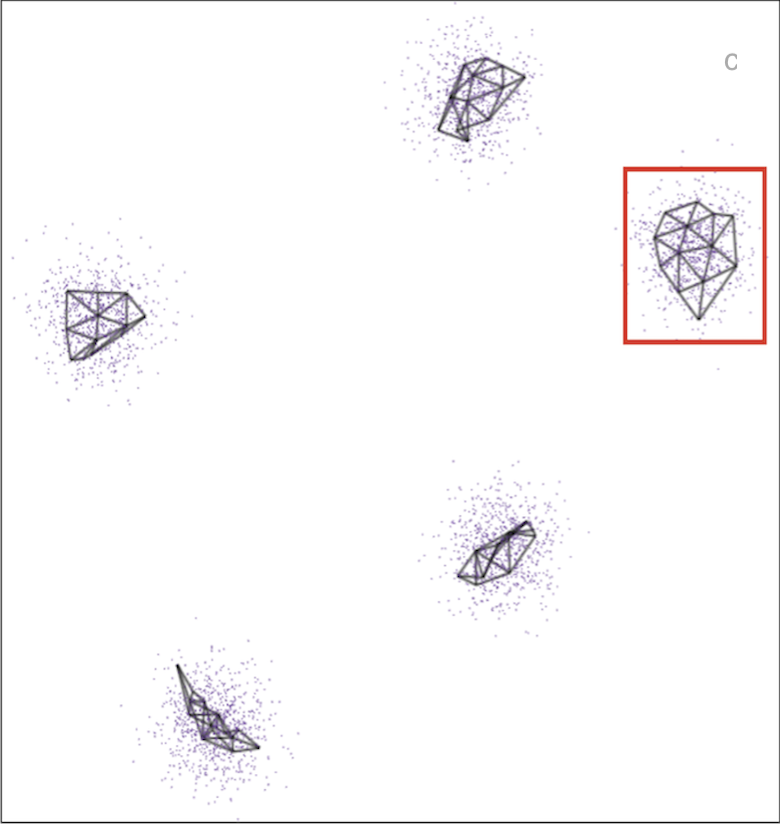
\includegraphics{figures/five_gau_clusters/sc_pacmap_2.png}

}

}

\subcaption{\label{fig-gau5_sc2}}
\end{minipage}%
%
\begin{minipage}[t]{0.33\linewidth}

{\centering 

\raisebox{-\height}{

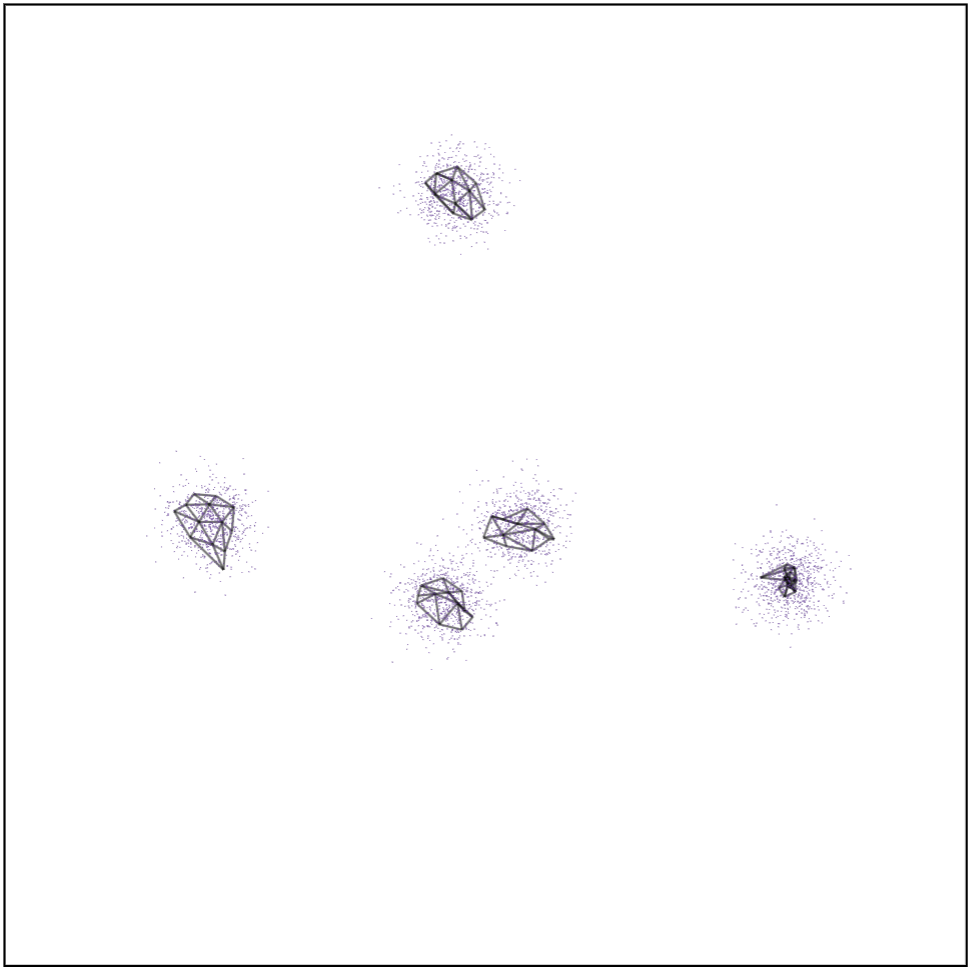
\includegraphics{figures/five_gau_clusters/sc_pacmap_3.png}

}

}

\subcaption{\label{fig-gau5_sc3}}
\end{minipage}%

\caption{\label{fig-gau5_sc}Screen shots of the \textbf{langevitour} of
the five Gaussian clusters dataset, shows the model with PaCMAP in
high-D, a video of the tour animation is available at
(\url{https://youtu.be/UxvU8HQd7JM}).}

\end{figure}

\hypertarget{sec-applications}{%
\section{Applications}\label{sec-applications}}

\hypertarget{single-cell-rna-seq-data-of-human}{%
\subsection{Single-cell RNA-seq data of
human}\label{single-cell-rna-seq-data-of-human}}

In the field of single-cell studies, a common analytical task involves
clustering to identify groups of cells with similar expression profiles.
Analysts often turn to NLDR techniques to verify and identify these
clusters and explore developmental trajectories. To illustrate the
importance of NLDR techniques and parameter selection in identifying
clusters, Human Peripheral Blood Mononclear Cells (PBMC3k) dataset
\citep{chen2023} is used. In a study by \citet{chen2023}, this dataset
was used to demonstrate how UMAP represents clusters (see
Figure~\ref{fig-umapauthor}). As shown in Figure~\ref{fig-umapauthor},
there are three distinct and well-separated clusters.

\begin{figure}[H]

{\centering 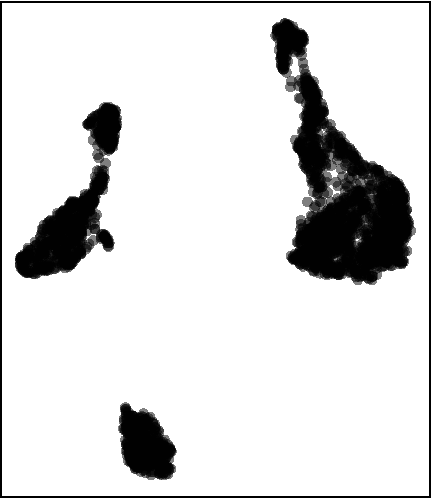
\includegraphics{paper_files/figure-pdf/fig-umapauthor-1.pdf}

}

\caption{\label{fig-umapauthor}2D layout from UMAP (n\_neighbors = 30,
min\_dist = 0.3) applied for the PBMC3k dataset. Is this a best
representation of the original data?}

\end{figure}

To determine whether the UMAP representation with the parameter choice
suggested by \citet{chen2023} preserves the original data structure, we
visualize the model constructed with UMAP overlaid on the high-D data
(model-in-data space). The figures in Figure~\ref{fig-pbmc1_sc} show
three well-separated clusters, indicating that the suggested UMAP
representation preserves the global structure (see
Figure~\ref{fig-umapauthor}). However, as shown in
Figure~\ref{fig-pbmc1_sc}, these clusters are close to each other in
high-D space. Also, nonlinear continuity patterns and high-density
patches within the clusters are observed (see
Figure~\ref{fig-pbmc1_sc}). Therefore, the suggested UMAP representation
(see Figure~\ref{fig-umapauthor}) does not accurately preserve the local
structure of the PBMC3k dataset.

\begin{figure}[H]

{\centering 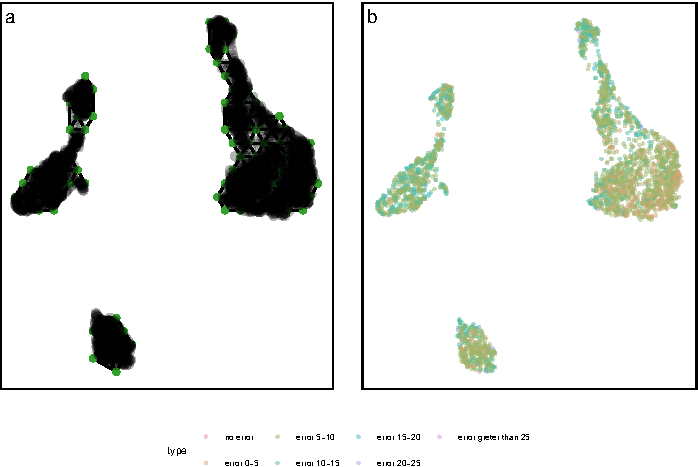
\includegraphics{paper_files/figure-pdf/fig-nldervisPBMCUMAP-1.pdf}

}

\caption{\label{fig-nldervisPBMCUMAP}(a) Model generated with 21 and 28
bins along x and y axes with hexagonal size 0.03 in the 2D space
overlaid on UMAP data, and (b) high-D model error in model space.}

\end{figure}

\begin{figure}[H]

\begin{minipage}[t]{0.33\linewidth}

{\centering 

\raisebox{-\height}{

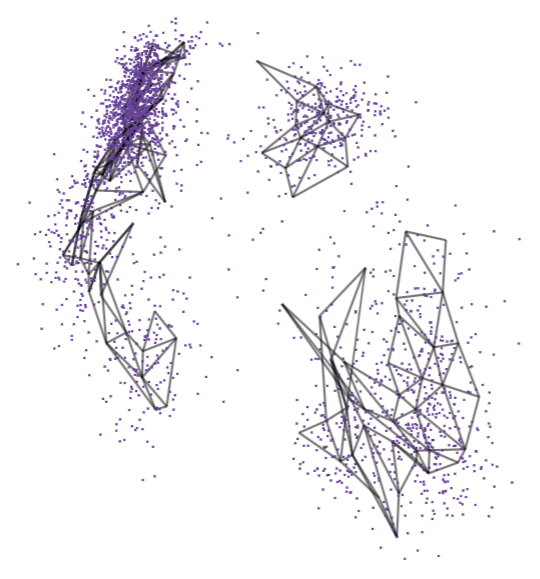
\includegraphics{figures/pbmc3k/sc_1.png}

}

}

\subcaption{\label{fig-pbmc1_sc1}}
\end{minipage}%
%
\begin{minipage}[t]{0.33\linewidth}

{\centering 

\raisebox{-\height}{

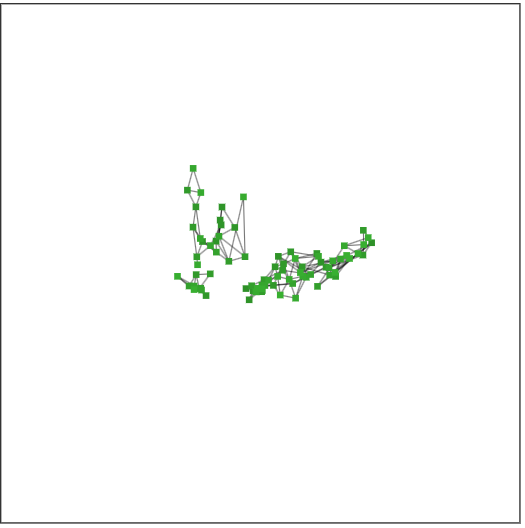
\includegraphics{figures/pbmc3k/sc_2.png}

}

}

\subcaption{\label{fig-pbmc1_sc2}}
\end{minipage}%
%
\begin{minipage}[t]{0.33\linewidth}

{\centering 

\raisebox{-\height}{

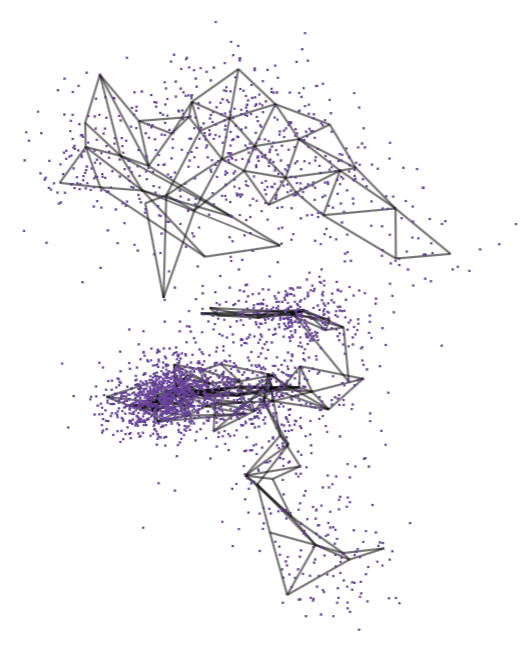
\includegraphics{figures/pbmc3k/sc_3.png}

}

}

\subcaption{\label{fig-pbmc1_sc3}}
\end{minipage}%

\caption{\label{fig-pbmc1_sc}Screen shots of the \textbf{langevitour} of
the PBMC3k data set, shows the model in high-D, a video of the tour
animation is available at (\url{https://youtu.be/Gnhh4hfsbbg}).}

\end{figure}

To find the best NLDR representation for PBMC3k dataset, we observe the
absolute error for different number of non-empty bins and select the one
with the lowest error. As shown in Figure~\ref{fig-abserrorPBMC}, tSNE
with a perplexity set to \(51\), has the lowest error. Therefore, tSNE
with a perplexity of \(51\) is used as the best representation for
PBMC3k dataset.

\begin{figure}[H]

{\centering 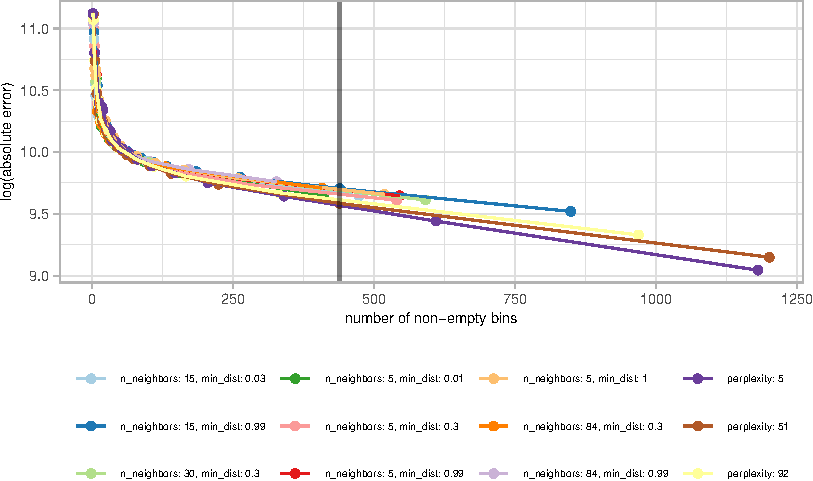
\includegraphics[width=1\textwidth,height=\textheight]{paper_files/figure-pdf/fig-abserrorPBMC-1.pdf}

}

\caption{\label{fig-abserrorPBMC}Absolute error from UMAP and tSNE
applied to training PBMC3k dataset with diffferent parameter choices.
What is the best parameter choice to create the model? The residual plot
have a steep slope at the beginning, indicating that a smaller number of
non-empty bins causes a larger amount of error. Then, the slope
gradually declines or level off, indicating that a higher number of
non-empty bins generates a smaller error. Using the elbow method, it was
observed that when the number of non-empty bins is set to 439, the
lowest error occurred with the parameters perplexity: 51.}

\end{figure}

As shown in Figure~\ref{fig-tsnesuggest}, there are three well-separated
clusters, although they are located close to each other. Additionally,
nonlinear structures can be observed within the clusters (see
Figure~\ref{fig-tsnesuggest}). Hence, the data structure that UMAP
failed to capture for the PBMC3k dataset is successfully captured by
tSNE.

\begin{figure}[H]

{\centering 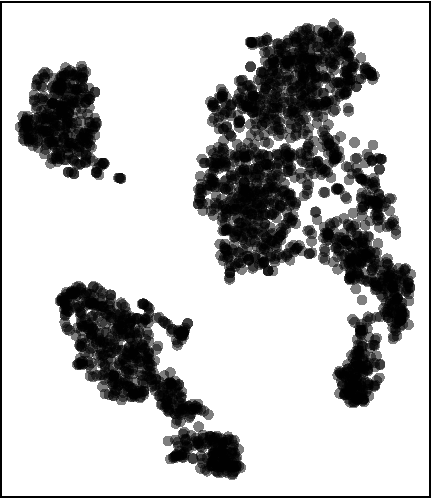
\includegraphics{paper_files/figure-pdf/fig-tsnesuggest-1.pdf}

}

\caption{\label{fig-tsnesuggest}2D layout from tSNE (perplexity = 51)
applied for the PBMC3k dataset. Is this a best representation of the
original data?}

\end{figure}

Next, the model is fitted for tSNE, and the resulting model is
visualized in the data space. The model shows some quirks, as shown in
Figure~\ref{fig-pbmc2_sc}. The large cluster is divided into three
subclusters, which are in close to each other.

\begin{figure}[H]

{\centering 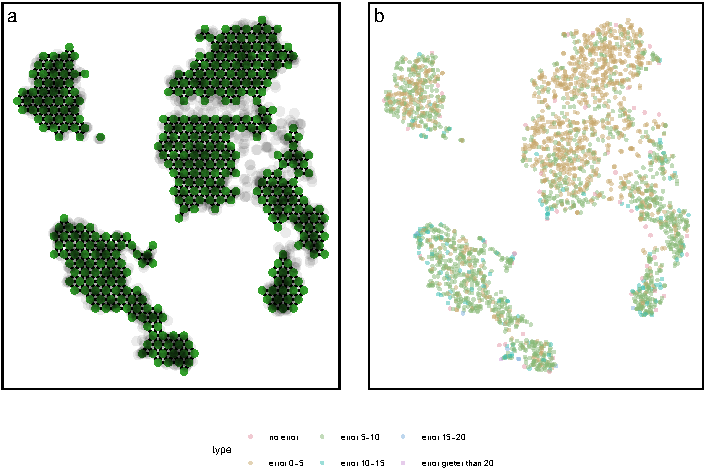
\includegraphics{paper_files/figure-pdf/fig-nldervisPBMCtSNE-1.pdf}

}

\caption{\label{fig-nldervisPBMCtSNE}(a) Model generated with 31 and 40
bins along x and y axes with hexagonal size 0.02 in the 2D space
overlaid on tSNE data, and (b) high-D model error in model space.}

\end{figure}

\begin{figure}[H]

\begin{minipage}[t]{0.33\linewidth}

{\centering 

\raisebox{-\height}{

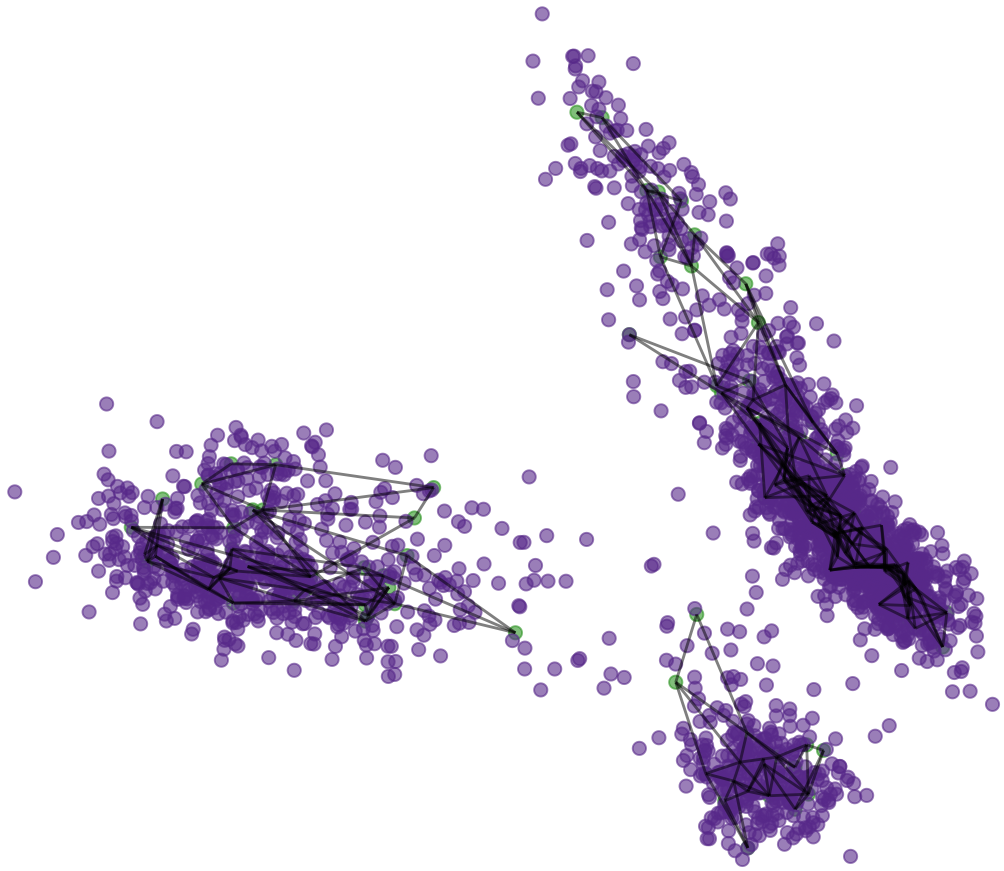
\includegraphics{figures/pbmc3k/sc_4.png}

}

}

\subcaption{\label{fig-pbmc2_sc4}}
\end{minipage}%
%
\begin{minipage}[t]{0.33\linewidth}

{\centering 

\raisebox{-\height}{

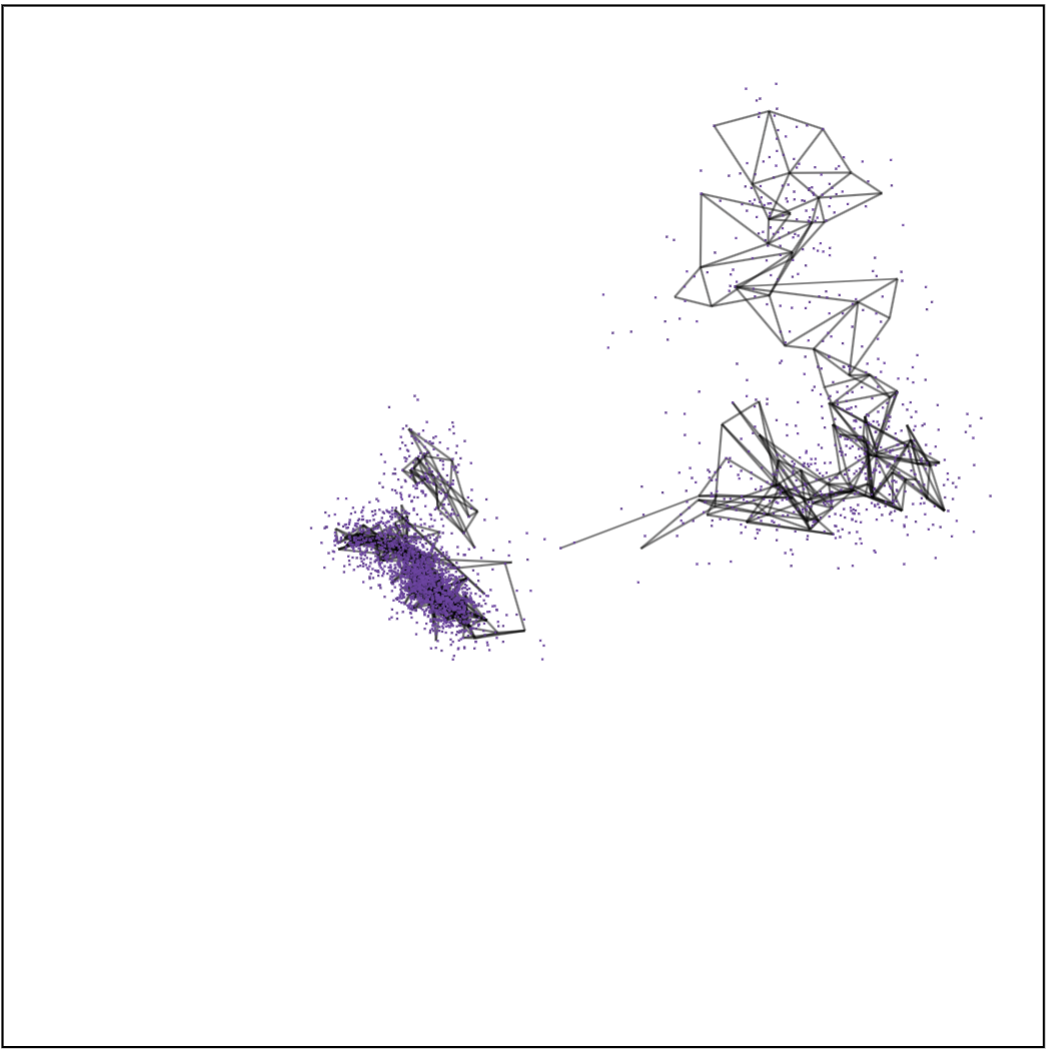
\includegraphics{figures/pbmc3k/sc_5.png}

}

}

\subcaption{\label{fig-pbmc2_sc5}}
\end{minipage}%
%
\begin{minipage}[t]{0.33\linewidth}

{\centering 

\raisebox{-\height}{

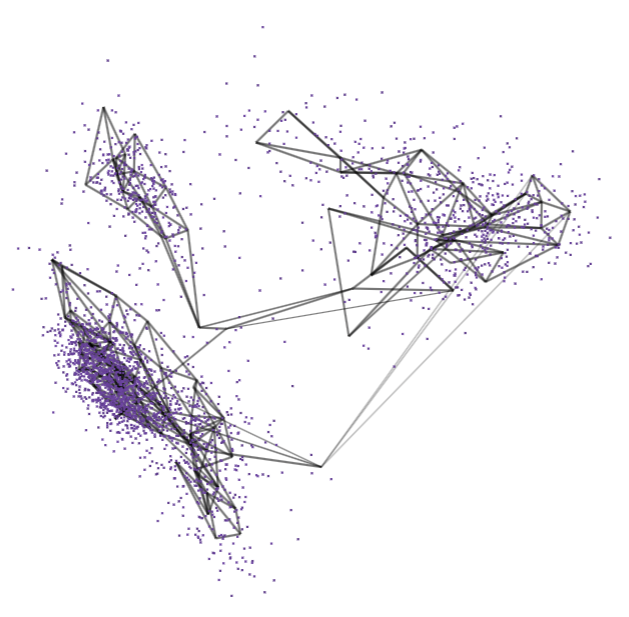
\includegraphics{figures/pbmc3k/sc_6.png}

}

}

\subcaption{\label{fig-pbmc2_sc6}}
\end{minipage}%

\caption{\label{fig-pbmc2_sc}Screen shots of the \textbf{langevitour} of
the PBMC3k data set, shows the model in high-D, a video of the tour
animation is available at (\url{https://youtu.be/R0EroJcGbas}).}

\end{figure}

\hypertarget{handwritten-digits}{%
\subsection{Handwritten digits}\label{handwritten-digits}}

The MNIST dataset consists of grayscale images of handwritten digits
\citep{lecun2010}. \citet{Yingfan2021} used this dataset to demonstrate
how the PaCMAP preserves local structure. We selected the 2D embedding
of PaCMAP for the handwritten digit 1. As shown in
Figure~\ref{fig-pacmapauthor}, we observe a nonlinear structure present
in 2D space. Furthermore, the angle of digit 1 images varies along the
nonlinear structure (see Figure~\ref{fig-sampleimg}). To answer the
following questions,

\begin{itemize}
\tightlist
\item
  Is the original data structure of the handwritten digit 1 dataset
  nonlinear?
\item
  Where does PaCMAP preserve the original data structure?
\item
  Where does PaCMAP show quirks?
\end{itemize}

we visualize the model constructed with PaCMAP overlaid on data in
high-D space (model-in-data space).

According to Figure~\ref{fig-mnist1_sc1}, the nonlinear continuity
structure observed in the 2D representation of PaCMAP is also visible
when visualizing the model overlaid on the data space. This provides
evidence that the model accurately captures the structure of the high-D
data. Also, the model has a twisted pattern within the nonlinear
structure, which is an addition pattern of data that cannot be seen in
the 2D representation (see Figure~\ref{fig-mnist1_sc2}).

In order to visually assess the preservation of local structure, it's
important to consider the edges in the model. In a model that
effectively preserves local structure, there shouldn't be any long edges
in high-D space. However, as shown in Figure~\ref{fig-mnist1_sc3}, some
long edges exist in high-D space that are not identified as long edges
in the 2D representation.

\begin{figure}[H]

{\centering 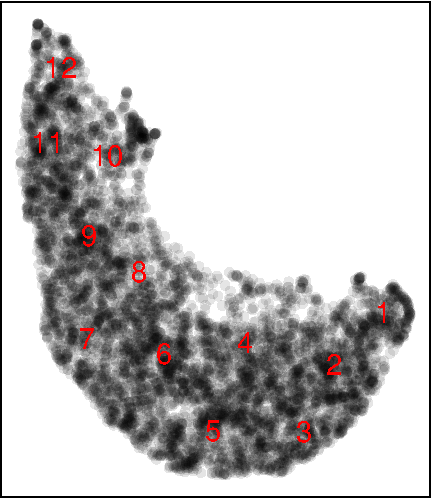
\includegraphics{paper_files/figure-pdf/fig-pacmapauthor-1.pdf}

}

\caption{\label{fig-pacmapauthor}(a) 2D layout from PaCMAP
(n\_components=2, n\_neighbors=10, init=random, MN\_ratio=0.9,
FP\_ratio=2.0) applied for the digit 1 of the MNIST dataset. Is this a
best representation of the original data?}

\end{figure}

\begin{figure}[H]

{\centering 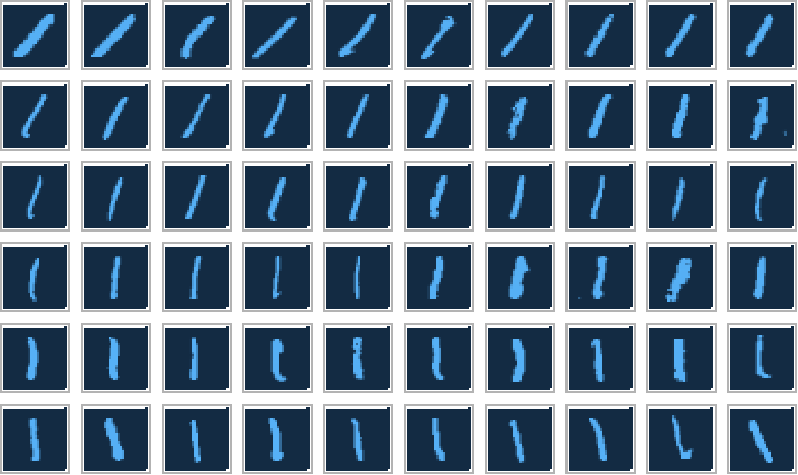
\includegraphics[width=1\textwidth,height=\textheight]{paper_files/figure-pdf/fig-sampleimg-1.pdf}

}

\caption{\label{fig-sampleimg}Images of the handwritten digit 1 are
distributed along the right-to-left of first embedding axis of the
PaCMAP nonlinear structure.}

\end{figure}

\begin{figure}[H]

{\centering 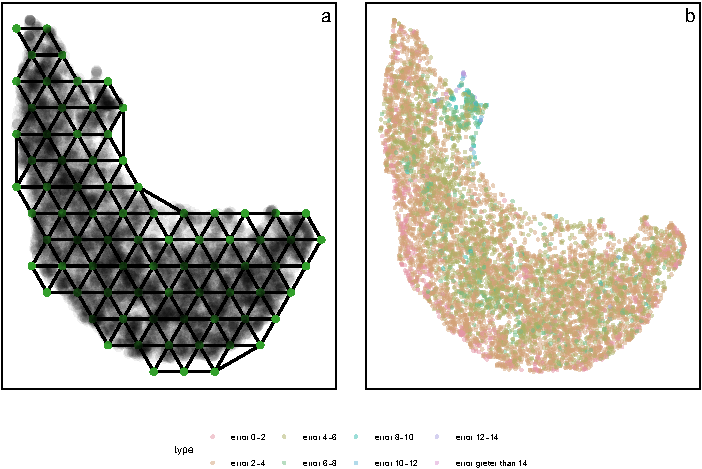
\includegraphics{paper_files/figure-pdf/fig-nldervisMNISTPACMAP-1.pdf}

}

\caption{\label{fig-nldervisMNISTPACMAP}(a) Model generated with 12 and
15 bins along x and y axes with hexagonal size 0.06 in the 2D space
overlaid on PaCMAP data, and (b) high-D model error in model space.}

\end{figure}

\begin{figure}[H]

\begin{minipage}[t]{0.33\linewidth}

{\centering 

\raisebox{-\height}{

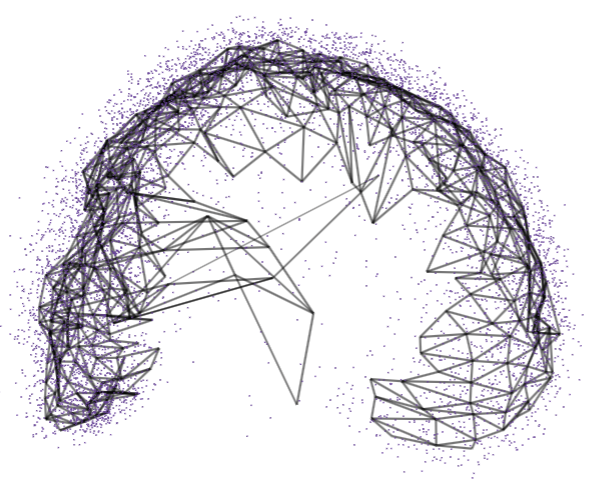
\includegraphics{figures/mnist/sc_1.png}

}

}

\subcaption{\label{fig-mnist1_sc1}}
\end{minipage}%
%
\begin{minipage}[t]{0.33\linewidth}

{\centering 

\raisebox{-\height}{

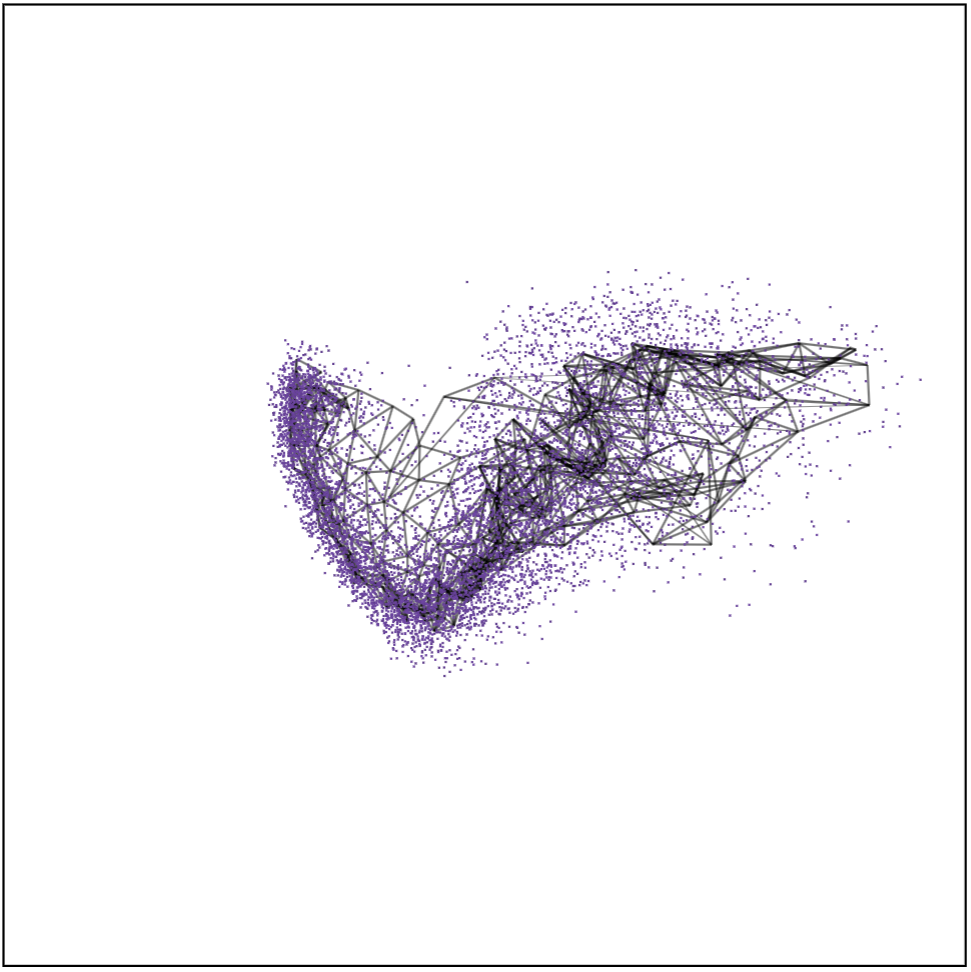
\includegraphics{figures/mnist/sc_2.png}

}

}

\subcaption{\label{fig-mnist1_sc2}}
\end{minipage}%
%
\begin{minipage}[t]{0.33\linewidth}

{\centering 

\raisebox{-\height}{

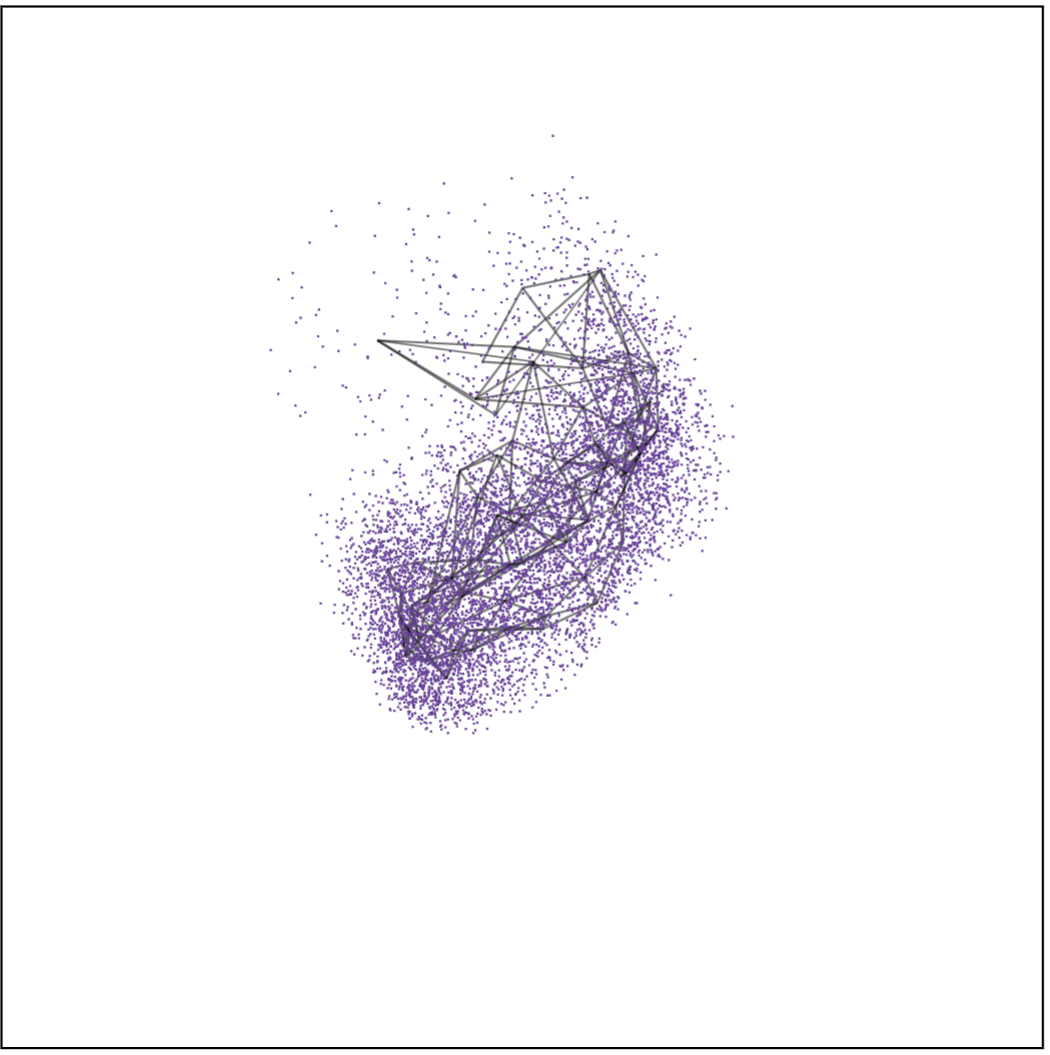
\includegraphics{figures/mnist/sc_3.png}

}

}

\subcaption{\label{fig-mnist1_sc3}}
\end{minipage}%

\caption{\label{fig-mnist1_sc}Screen shots of the \textbf{langevitour}
of the MNIST digit 1 data set, shows the model-in-data space, a video of
the tour animation is available at
(\url{https://youtu.be/zq2GM9qvUNA}).}

\end{figure}

In terms of model error, some data points show high error (see
Figure~\ref{fig-nldervisMNISTPACMAP}) due to their deviation from the
typical high-D data structure, acting as outliers. This is evident when
comparing the images associated with these high model error points (see
Figure~\ref{fig-sampleimgerror}) to others (see
Figure~\ref{fig-sampleimg}).

\begin{figure}[H]

{\centering 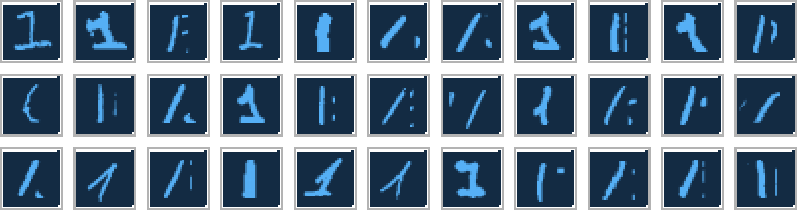
\includegraphics[width=1\textwidth,height=\textheight]{paper_files/figure-pdf/fig-sampleimgerror-1.pdf}

}

\caption{\label{fig-sampleimgerror}Images of handwritten digit 1 which
occur large model error.}

\end{figure}

\hypertarget{sec-conclusion}{%
\section{Conclusion}\label{sec-conclusion}}

In conclusion, our proposed model offers a novel approach for
visualizing high-dimensional (high-D) data by leveraging non-linear
dimension reduction (NLDR) techniques. Through a series of steps
including hexagonating NLDR data, triangulating bin centroids, and
lifting the 2D triangular mesh into high dimensions, our model
effectively transforms complex high-D data into interpretable 2D
representations. The model's performance is evaluated using goodness of
fit statistics such as Mean Squared Error (MSE) and Akaike Information
Criterion (AIC), providing insights into its accuracy and reliability.
Overall, our model presents a valuable tool for researchers and
practitioners in various fields to gain deeper insights from
high-dimensional datasets.

Our algorithm mainly consists\ldots{}

These Goodness of fit statistics useful in encountering the prediction
accuracy when we predict the 2D embedding for the new high-D data.
Because, we try to find the nearest high-D mappings as the first step of
prediction which will participate the prediction process. When we need
to find which different NLDR technique and which parameter choices is
giving the best representation of high-D data, MSE and AIC are also
useful.

We introduce a new tool to help to determine which method, which
parameter choice provide the most useful representation of high-D data.

\hypertarget{references}{%
\section*{References}\label{references}}
\addcontentsline{toc}{section}{References}

\renewcommand{\bibsection}{}
\bibliography{bibliography.bib}

\newpage{}




\end{document}
